\documentclass[11pt]{article} % use larger type; default would be 10pt

\usepackage{pgfplots}
\usetikzlibrary{calc}
\usetikzlibrary{arrows}
\usetikzlibrary{patterns}
\usetikzlibrary{calc,intersections,through,backgrounds}
\usetikzlibrary{decorations.pathreplacing}
        \newcommand\degree[0]{^{\circ}}
        \newcommand\abs[1]{\left|#1\right|}

\title{Play with TikZ}
\author{Just Us}
%\date{} % Activate to display a given date or no date (if empty),
         % otherwise the current date is printed 

\begin{document}
\maketitle

\section{Chap 1 Section 1}

Example 3 fig-1-1-1

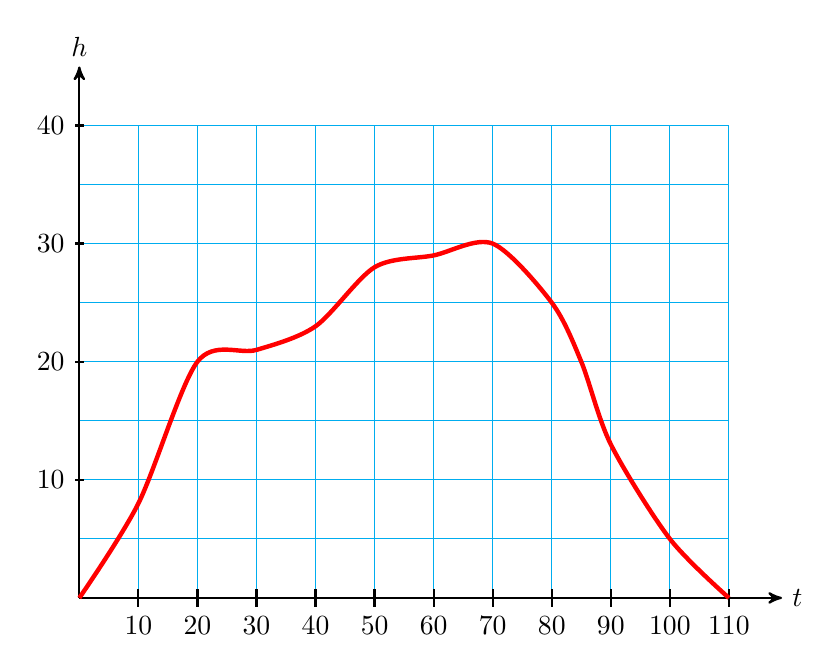
\begin{tikzpicture} [xscale=.075, yscale=.15]
\draw[cyan] (0,0) grid[xstep=10, ystep=5] (110,40);
\draw[black,thick, ->, >=stealth'] (0,0)--(119,0) node[right]{$t$};
\draw[black,thick, ->, >=stealth'] (0,0)--(0,45) node[above]{$h$};
\foreach \x in  {10, 20, ..., 110} {
 \draw[black, thick] (\x,.75) --++(0,-1.5)  node[below]   {\x};
}
\foreach \y in  {10, 20, ..., 40} {
 \draw[black, thick] (.75,\y) --++(-1.5,0)  node[left]   {\y};
}
\draw [red, ultra thick] plot [smooth] coordinates {(0,0) (10,8) (20,20) (30,21) (40,23) (50,28) (60,29) (70,30) (80,25) (85,20) (90,13) (100,5) (110,0) };
\end{tikzpicture}
\newline


Example 4 fig-1-1-ex4

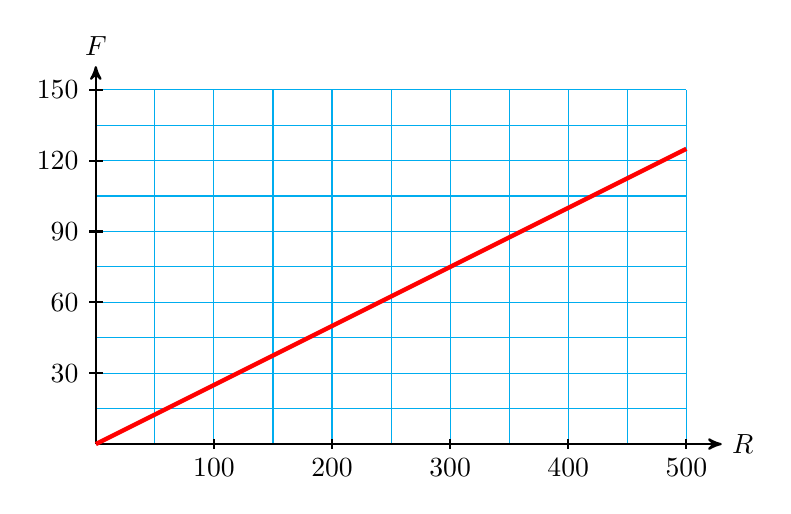
\begin{tikzpicture} [xscale=.015, yscale=.03]
\draw[cyan] (0,0) grid[xstep=50, ystep=15] (500,150);
\draw[black,thick, ->, >=stealth'] (0,0)--(530,0) node[right]{$R$};
\draw[black,thick, ->, >=stealth'] (0,0)--(0,160) node[above]{$F$};
\foreach \x in  {100, 200, ..., 500} {
 \draw[black, thick] (\x,2) --++(0,-4)  node[below]   {\x};
}
\foreach \y in  {30, 60, ..., 150} {
 \draw[black, thick] (6,\y) --++(-12,0)  node[left]   {\y};
}
\draw [red, ultra thick] (0,0) -- (500,125);
\end{tikzpicture}
\newline




Example 3 fig-1-1-ex3

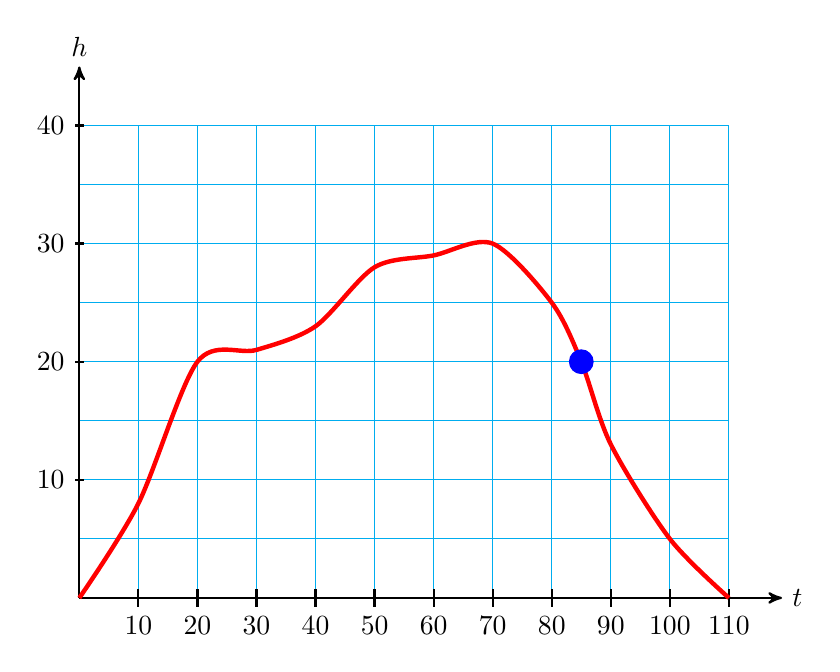
\begin{tikzpicture} [xscale=.075, yscale=.15]
\draw[cyan] (0,0) grid[xstep=10, ystep=5] (110,40);
\draw[black,thick, ->, >=stealth'] (0,0)--(119,0) node[right]{$t$};
\draw[black,thick, ->, >=stealth'] (0,0)--(0,45) node[above]{$h$};
\foreach \x in  {10, 20, ..., 110} {
 \draw[black, thick] (\x,.75) --++(0,-1.5)  node[below]   {\x};
}
\foreach \y in  {10, 20, ..., 40} {
 \draw[black, thick] (.75,\y) --++(-1.5,0)  node[left]   {\y};
}
\draw [red, ultra thick] plot [smooth] coordinates {(0,0) (10,8) (20,20) (30,21) (40,23) (50,28) (60,29) (70,30) (80,25) (85,20) (90,13) (100,5) (110,0) };
\draw[blue, fill=blue] (85,20) ellipse (2cm and 1cm);
\end{tikzpicture}
\newline

sw-1-3-1 number line

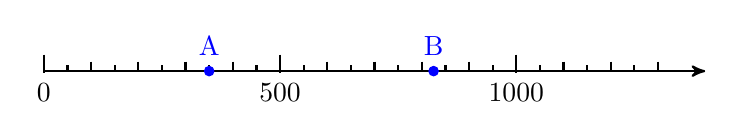
\begin{tikzpicture} [scale=.6]
\draw[black,thick, ->, >=stealth'] (0,0)--(14,0);
\foreach \x [evaluate=\x as \xi using int(100*\x)] in  {0,5,10} {
 \draw[black, thick] (\x,.35) --++(0,-.4)  node[below]   {\xi};
}
\foreach \x in {1,2,...,13} \draw[black,thick] (\x,.2) --++(0,-.2);
\foreach \x in {1,2,...,13} \draw[black,thick] ({\x-1/2},.12) --++(0,-.12);
\filldraw[blue] (3.5,0) circle (1mm) node[above, yshift=2] {A};
\filldraw[blue] (8.25,0) circle (1mm) node[above, yshift=2] {B};

\end{tikzpicture}
\newline

sw-1-3-2 number line

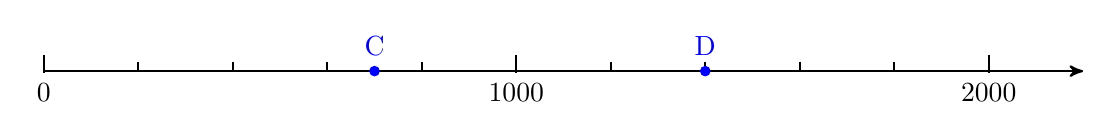
\begin{tikzpicture} [scale=.6]
\draw[black,thick, ->, >=stealth'] (0,0)--(22,0);
\foreach \x [evaluate=\x as \xi using int(100*\x)] in  {0,10,20} {
 \draw[black, thick] (\x,.35) --++(0,-.4)  node[below]   {\xi};
}
\foreach \x in {2,4,...,20} \draw[black,thick] (\x,.2) --++(0,-.2);
\filldraw[blue] (7,0) circle (1mm) node[above, yshift=2] {C};
\filldraw[blue] (14,0) circle (1mm) node[above, yshift=2] {D};

\end{tikzpicture}
\newline

sw-1-3-3 number line

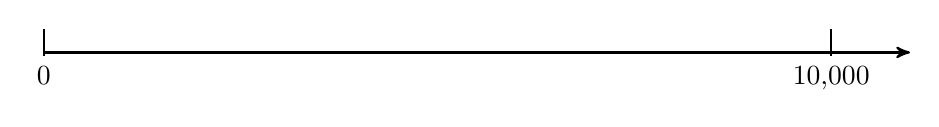
\begin{tikzpicture} 
\draw[black,thick, ->, >=stealth'] (0,0)--(11,0);
 \draw[black, thick] (0,.3) --++(0,-.35)  node[below]   {0};
 \draw[black, thick] (10,.3) --++(0,-.35)  node[below]   {10,000};

\end{tikzpicture}
\newline

sw-1-3-3ans number line

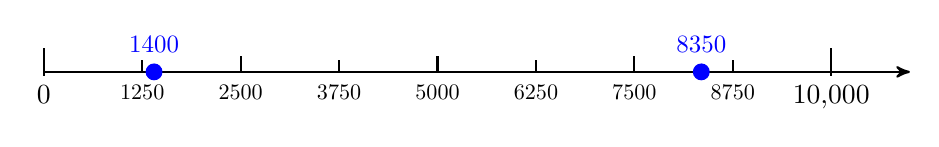
\begin{tikzpicture} 
\draw[black,thick, ->, >=stealth'] (0,0)--(11,0);
 \draw[black, thick] (0,.3) --++(0,-.35)  node[below]   {0};
 \draw[black, thick] (10,.3) --++(0,-.35)  node[below]   {10,000};
\foreach \x [evaluate=\x as \xi using int(1000*\x)] in {5/2,5,15/2} \draw[black,thick] (\x,.2) --++(0,-.2) node[below, yshift=-2, scale=.8]{\xi};
\foreach \x [evaluate=\x as \xi using int(1000*\x)]  in {1.25, 3.75, 6.25, 8.75} \draw[black,thick] (\x,.15) --++(0,-.15) node[below, yshift=-2, scale=.8]{\xi};
\filldraw[blue] (1.4,0) circle (1mm) node[above, yshift=4, scale=.9] {1400};
\filldraw[blue] (8.35,0) circle (1mm) node[above, yshift=4, scale=.9] {8350};

\end{tikzpicture}
\newline

sw-1-3-4 number line

\begin{tikzpicture}  [scale=.8]
\draw[black,thick, ->, >=stealth'] (0,0)--(16.5,0);
\draw[black, thick] (0,.3) --++(0,-.35)  node[below]   {0};

\end{tikzpicture}
\newline

sw-1-3-4ans number line

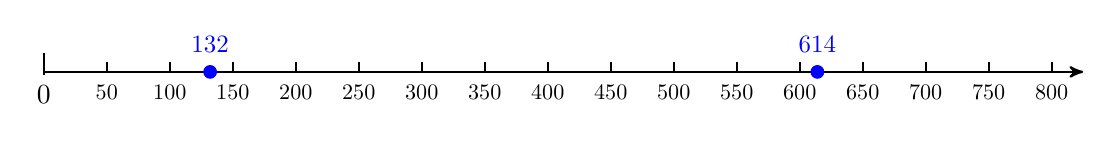
\begin{tikzpicture}  [scale=.8]
\draw[black,thick, ->, >=stealth'] (0,0)--(16.5,0);
\draw[black, thick] (0,.3) --++(0,-.35)  node[below]   {0};
\foreach \x [evaluate=\x as \xi using int(50*\x)]  in {1,2,...,16} \draw[black,thick] (\x,.15) --++(0,-.15) node[below, yshift=-2, scale=.8]{\xi};
\filldraw[blue] (2.64,0) circle (1mm) node[above, yshift=4, scale=.9] {132};
\filldraw[blue] (12.28,0) circle (1mm) node[above, yshift=4, scale=.9] {614};

\end{tikzpicture}
\newline

sw-1-3-5ans number line

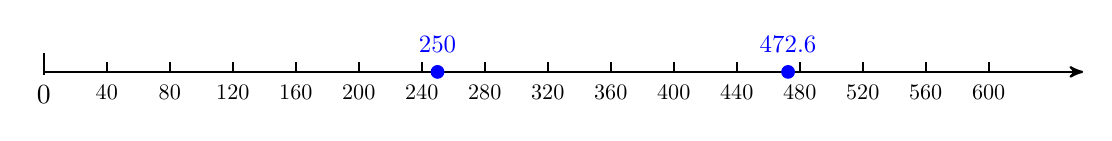
\begin{tikzpicture}  [scale=.8]
\draw[black,thick, ->, >=stealth'] (0,0)--(16.5,0);
\draw[black, thick] (0,.3) --++(0,-.35)  node[below]   {0};
\foreach \x [evaluate=\x as \xi using int(40*\x)]  in {1,2,...,15} \draw[black,thick] (\x,.15) --++(0,-.15) node[below, yshift=-2, scale=.8]{\xi};
\filldraw[blue] (6.25,0) circle (1mm) node[above, yshift=4, scale=.9] {250};
\filldraw[blue] (11.815,0) circle (1mm) node[above, yshift=4, scale=.9] {472.6};

\end{tikzpicture}
\newline

sw-1-3-6ans number line

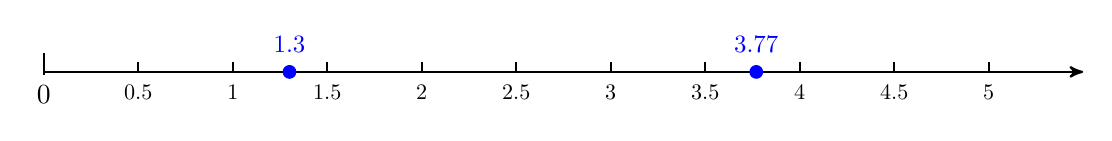
\begin{tikzpicture}  [scale=.8]
\draw[black,thick, ->, >=stealth'] (0,0)--(16.5,0);
\draw[black, thick] (0,.3) --++(0,-.35)  node[below]   {0};
\foreach \x [evaluate=\x as \xi using int(\x/3)]  in {3,6,...,15} \draw[black,thick] (\x,.15) --++(0,-.15) node[below, yshift=-2, scale=.8]{\xi};
\foreach \x [evaluate=\x as \xi using int(\x/3)]  in {1.5,4.5,...,13.5} \draw[black,thick] (\x,.15) --++(0,-.15) node[below, yshift=-2, scale=.8]{\xi.5};
\filldraw[blue] (3.9,0) circle (1mm) node[above, yshift=4, scale=.9] {1.3};
\filldraw[blue] (11.31,0) circle (1mm) node[above, yshift=4, scale=.9] {3.77};

\end{tikzpicture}
\newline



hp-1-1-9 grid

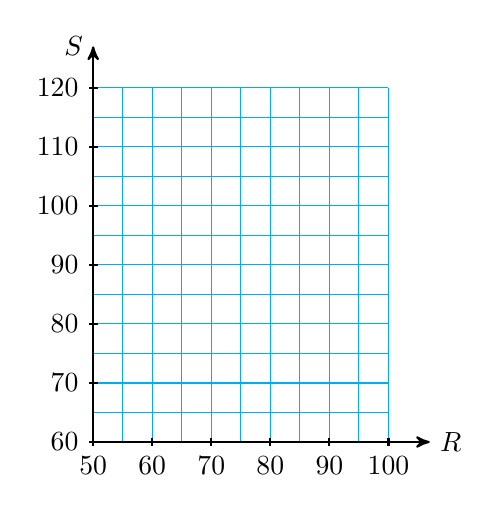
\begin{tikzpicture} [xscale=.075, yscale=.075]
\draw[cyan] (50,60) grid[step=5] (100,120);
\draw[black,thick, ->, >=stealth'] (50,60)--(107,60) node[right]{$R$};
\draw[black,thick, ->, >=stealth'] (50,60)--(50,127) node[left]{$S$};
\foreach \x in  {50, 60, ..., 100} {
 \draw[black, thick] (\x,60.75) --++(0,-1.5)  node[below]   {\x};
}
\foreach \y in  {60, 70, ..., 120} {
 \draw[black, thick] (50.75,\y) --++(-1.5,0)  node[left]   {\y};
}
\end{tikzpicture}
\newline


hp-1-1-9ans line

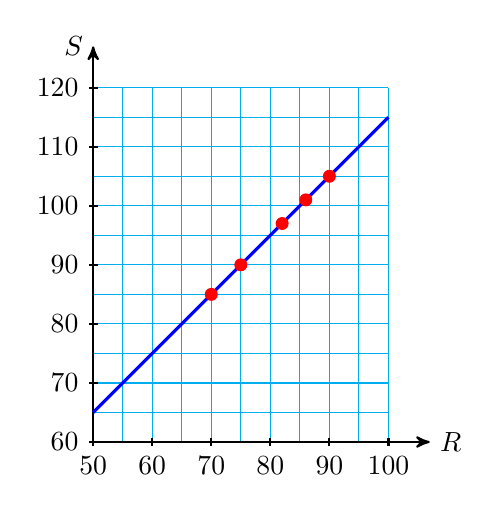
\begin{tikzpicture} [xscale=.075, yscale=.075]
\draw[cyan] (50,60) grid[step=5] (100,120);
\draw[black,thick, ->, >=stealth'] (50,60)--(107,60) node[right]{$R$};
\draw[black,thick, ->, >=stealth'] (50,60)--(50,127) node[left]{$S$};
\foreach \x in  {50, 60, ..., 100} {
 \draw[black, thick] (\x,60.75) --++(0,-1.5)  node[below]   {\x};
}
\foreach \y in  {60, 70, ..., 120} {
 \draw[black, thick] (50.75,\y) --++(-1.5,0)  node[left]   {\y};
}
\draw[blue, very thick] (50,65)--(100,115);
\foreach \x in {70, 75, 82, 86, 90}{
 \draw[red, fill=red] (\x, {\x+15}) circle (1cm);
 }
\end{tikzpicture}
\newline


hp-1-1-10 grid

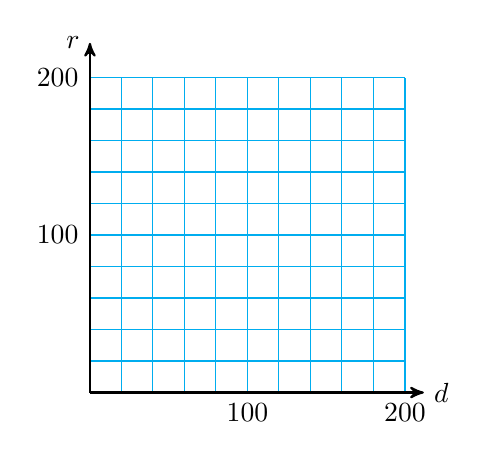
\begin{tikzpicture} [scale=.02]
\draw[cyan] (0,0) grid[step=20] (200,200);
\draw[black,thick, ->, >=stealth'] (0,0)--(212,0) node[right]{$d$};
\draw[black,thick, ->, >=stealth'] (0,0)--(0,222) node[left]{$r$};
\foreach \x in  {100,200} {
 \draw[black, thick] (\x,0.75) --++(0,-1.5)  node[below]   {\x};
 \draw[black, thick] (0.75,\x) --++(-1.5,0)  node[left]   {\x};
}
\end{tikzpicture}
\newline



hp-1-1-11 grid

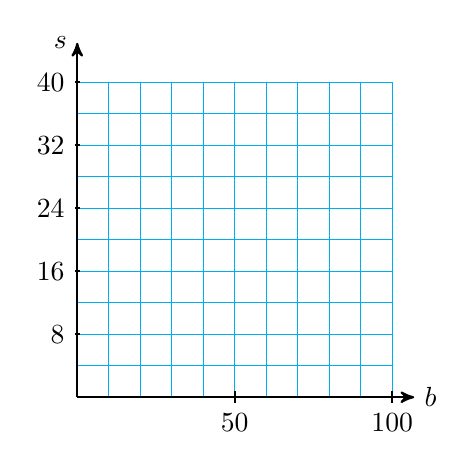
\begin{tikzpicture} [xscale=.04, yscale=0.1]
\draw[cyan] (0,0) grid[xstep=10, ystep=4] (100,40);
\draw[black,thick, ->, >=stealth'] (0,0)--(107,0) node[right]{$b$};
\draw[black,thick, ->, >=stealth'] (0,0)--(0,45) node[left]{$s$};
\foreach \x in  {50, 100} {
 \draw[black, thick] (\x,0.75) --++(0,-1.5)  node[below]   {\x};
}
\foreach \y in  {8,16, ..., 40} {
 \draw[black, thick] (0.75,\y) --++(-1.5,0)  node[left]   {\y};
}
\end{tikzpicture}
\newline



hp-1-1-11ans line

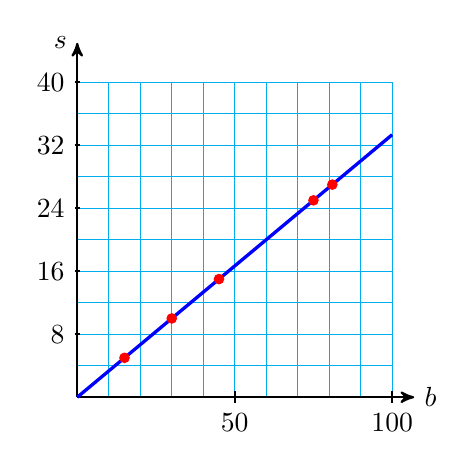
\begin{tikzpicture} [xscale=.04, yscale=0.1]
\draw[cyan] (0,0) grid[xstep=10, ystep=4] (100,40);
\draw[black,thick, ->, >=stealth'] (0,0)--(107,0) node[right]{$b$};
\draw[black,thick, ->, >=stealth'] (0,0)--(0,45) node[left]{$s$};
\foreach \x in  {50, 100} {
 \draw[black, thick] (\x,0.75) --++(0,-1.5)  node[below]   {\x};
}
\foreach \y in  {8,16, ..., 40} {
 \draw[black, thick] (0.75,\y) --++(-1.5,0)  node[left]   {\y};
}
\draw[blue, very thick] (0,0)--(100,100/3);
\foreach \x in {15, 30, 45, 75, 81}{
 \draw[red, fill=red] (\x, {\x/3}) ellipse (1.5cm and 0.6cm);
 }
\end{tikzpicture}
\newline



hp-1-1-12 grid

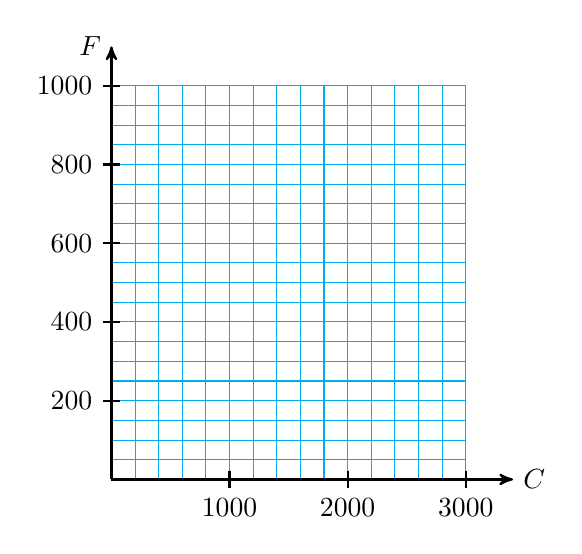
\begin{tikzpicture} [xscale = 1.5, yscale=0.5]
\draw[cyan] (0,0) grid[xstep=0.2, ystep=.5] (3,10);
\draw[black,thick, ->, >=stealth'] (0,0)--(3.40,0) node[right]{$C$};
\draw[black,thick, ->, >=stealth'] (0,0)--(0,11) node[left]{$F$};
\foreach \x [evaluate=\x as \xi using int( 1000* \x )]  in  {1,2,3} {
 \draw[black, thick] (\x,0.225) --++(0,-.45)  node[below]   {\xi};
}
\foreach \y [evaluate=\y as \yi using int( 100* \y )]  in  {2,4,..., 10} {
 \draw[black, thick] (0.075,\y) --++(-.15,0)  node[left]   {\yi};
}
\end{tikzpicture}
\newline




hp-1-1-13 retirement account

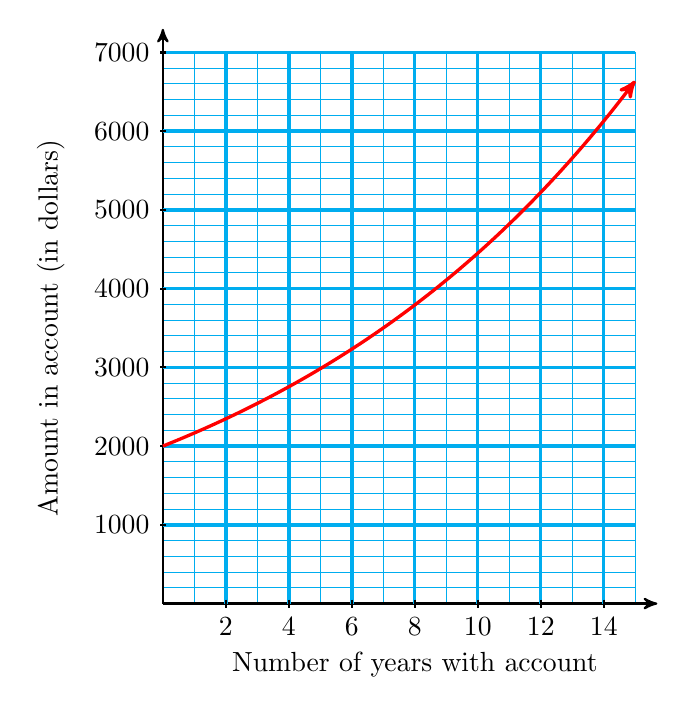
\begin{tikzpicture} [xscale = 0.4,]
\draw[cyan] (0,0) grid[xstep=1, ystep=.2] (15,7);
\draw[black,thick, ->, >=stealth'] (0,0)--(15.7,0);
\draw[black,thick, ->, >=stealth'] (0,0)--(0,7.3);
\foreach \x  in  {2,4,...,14} {
 \draw[cyan, very thick] (\x,0) --++(0,7);
 \draw[black, thick] (\x,0.05) --++(0,-.1)  node[below]   {\x};
}
\foreach \y [evaluate=\y as \yi using int( 1000* \y )]  in  {1,2,..., 7} {
 \draw[cyan, very thick] (0, \y) --++(15,0);
 \draw[black, thick] (0.1,\y) --++(-.2,0)  node[left]   {\yi};
}
\node[label=left:\rotatebox{90}{Amount in account (in dollars)}] at (-2.5,3.5) {};
\node[below] at (8,-.5) {Number of years with account};
\draw[samples=65,domain=0:15,smooth,variable=\x,red,very thick, ->, >=stealth'] plot ({\x},{2*e^(.08*\x)});
\end{tikzpicture}
\newline




hp-1-1-14 temperature of soup

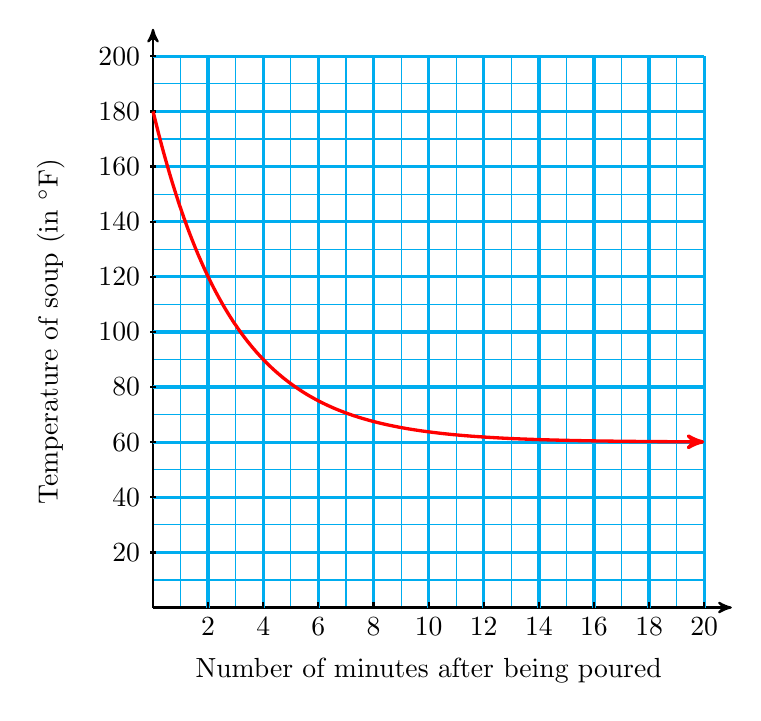
\begin{tikzpicture} [scale = 0.35]
\draw[cyan] (0,0) grid  (20,20);
\draw[black,thick, ->, >=stealth'] (0,0)--(21,0);
\draw[black,thick, ->, >=stealth'] (0,0)--(0,21);
\foreach \x  in  {2,4,...,20} {
 \draw[cyan, very thick] (\x,0) --++(0,20);
 \draw[black, thick] (\x,0.2) --++(0,-.2)  node[below]   {\x};
}
\foreach \y [evaluate=\y as \yi using int( 10* \y )]  in  {2,4,...,20} {
 \draw[cyan, very thick] (0, \y) --++(20,0);
 \draw[black, thick] (0.1,\y) --++(-.2,0)  node[left]   {\yi};
}
\node[label=left:\rotatebox{90}{Temperature of soup (in $\degree$F)}] at (-2.5,10) {};
\node[below] at (10,-1.5) {Number of minutes after being poured};
\draw[samples=65,domain=0:20,smooth,variable=\x,red,very thick, ->, >=stealth'] plot ({\x},{6+12*2^(-\x/2)});
\end{tikzpicture}
\newline





hp-1-1-15 four speed vs time graphs

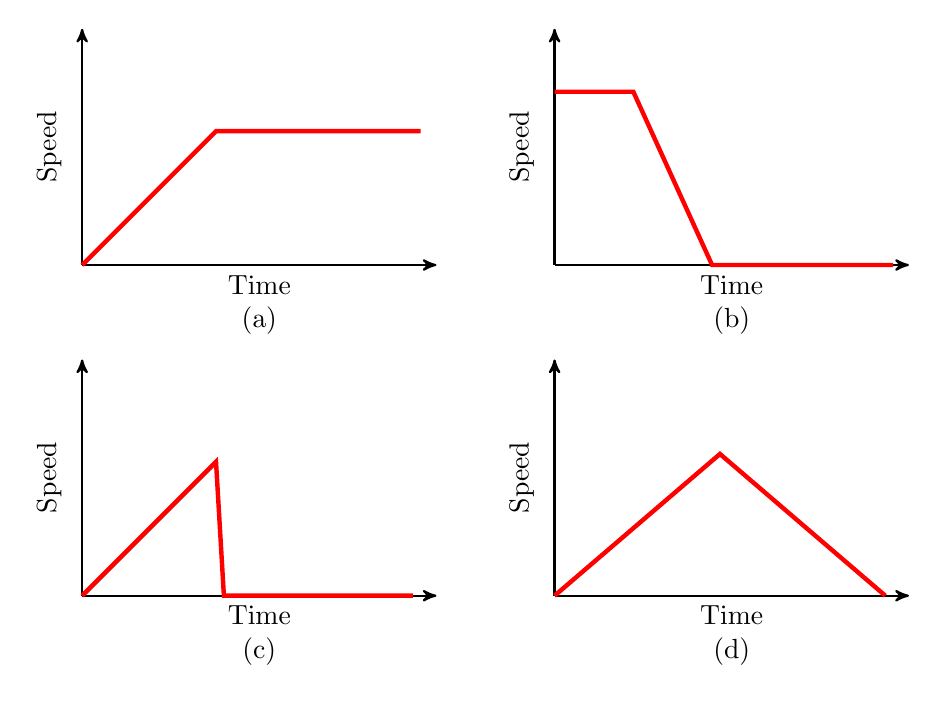
\begin{tikzpicture} 
\coordinate (O) at (0,0);
\draw[black,thick, ->, >=stealth'] (O)--++(4.5,0) node[below,midway, align=center]{Time\\(a)};;
\draw[black,thick, ->, >=stealth'] (O)--++(0,3) node[midway,label=left:\rotatebox{90}{Speed}]  {};;
\draw[red, ultra thick] (O)--++(1.7,1.7)--++(2.6,0);


\coordinate (O) at (6,0);
\draw[black,thick, ->, >=stealth'] (O)--++(4.5,0) node[below,midway, align=center]{Time\\(b)};
\draw[black,thick, ->, >=stealth'] (O)--++(0,3) node[midway,label=left:\rotatebox{90}{Speed}]  {};;
\draw[red, ultra thick] (O)++(0,2.2)--++(1,0)--++(1,-2.2)--++(2.3,0);


\coordinate (O) at (0,-4.2);
\draw[black,thick, ->, >=stealth'] (O)--++(4.5,0) node[below,midway, align=center]{Time\\(c)};;
\draw[black,thick, ->, >=stealth'] (O)--++(0,3) node[midway,label=left:\rotatebox{90}{Speed}]  {};;
\draw[red, ultra thick] (O)--++(1.7,1.7)--++(0.1,-1.7)--++(2.4,0);


\coordinate (O) at (6,-4.2);
\draw[black,thick, ->, >=stealth'] (O)--++(4.5,0) node[below,midway, align=center]{Time\\(d)};
\draw[black,thick, ->, >=stealth'] (O)--++(0,3) node[midway,label=left:\rotatebox{90}{Speed}]  {};;
\draw[red, ultra thick] (O)--++(2.1,1.8)--++(2.1,-1.8);
\end{tikzpicture}
\newline



hp-1-1-16 four distance vs time graphs

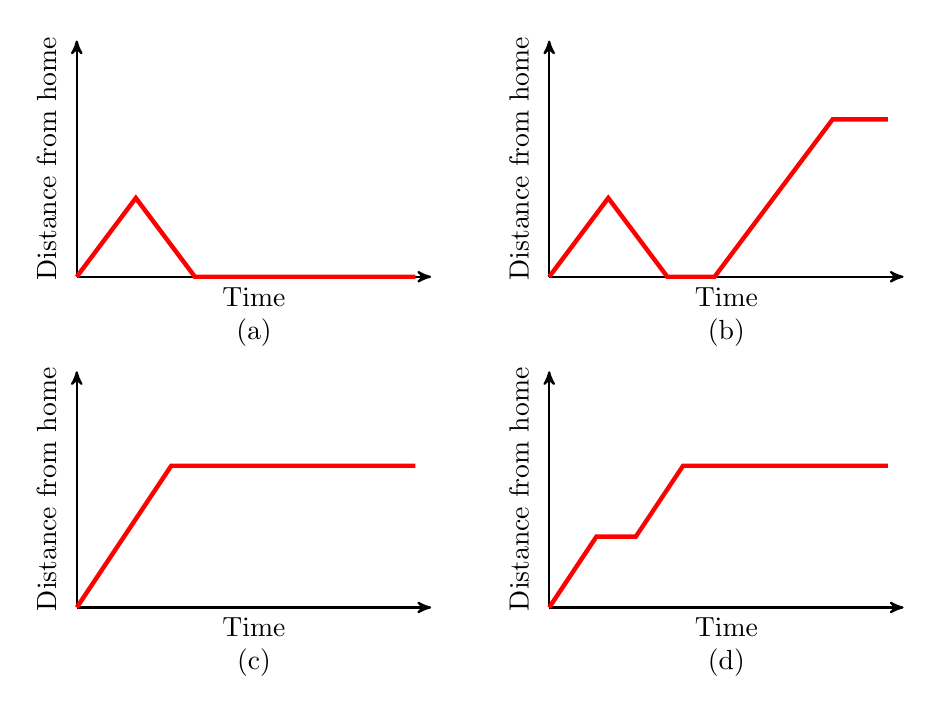
\begin{tikzpicture} 
\coordinate (O) at (0,0);
\draw[black,thick, ->, >=stealth'] (O)--++(4.5,0) node[below,midway, align=center]{Time\\(a)};;
\draw[black,thick, ->, >=stealth'] (O)--++(0,3) node[midway,label=left:\rotatebox{90}{Distance from home}]  {};;
\draw[red, ultra thick] (O)--++(.75,1.)--++(.75,-1.)--++(2.8,0);

\coordinate (O) at (6,0);
\draw[black,thick, ->, >=stealth'] (O)--++(4.5,0) node[below,midway, align=center]{Time\\(b)};
\draw[black,thick, ->, >=stealth'] (O)--++(0,3) node[midway,label=left:\rotatebox{90}{Distance from home}]  {};;
\draw[red, ultra thick] (O)--++(.75,1.)--++(.75,-1.)--++(0.6,0)--++(1.5,2)--++(0.7,0);

\coordinate (O) at (0,-4.2);
\draw[black,thick, ->, >=stealth'] (O)--++(4.5,0) node[below,midway, align=center]{Time\\(c)};;
\draw[black,thick, ->, >=stealth'] (O)--++(0,3) node[midway,label=left:\rotatebox{90}{Distance from home}]  {};;
\draw[red, ultra thick] (O)--++(1.2,1.8)--++(3.1,0);

\coordinate (O) at (6,-4.2);
\draw[black,thick, ->, >=stealth'] (O)--++(4.5,0) node[below,midway, align=center]{Time\\(d)};
\draw[black,thick, ->, >=stealth'] (O)--++(0,3) node[midway,label=left:\rotatebox{90}{Distance from home}]  {};;
\draw[red, ultra thick] (O)--++(0.6,0.9)--++(.5,0)--++(0.6,0.9)--++(2.6,0);
\end{tikzpicture}
\newline


hp-1-1-17a grid

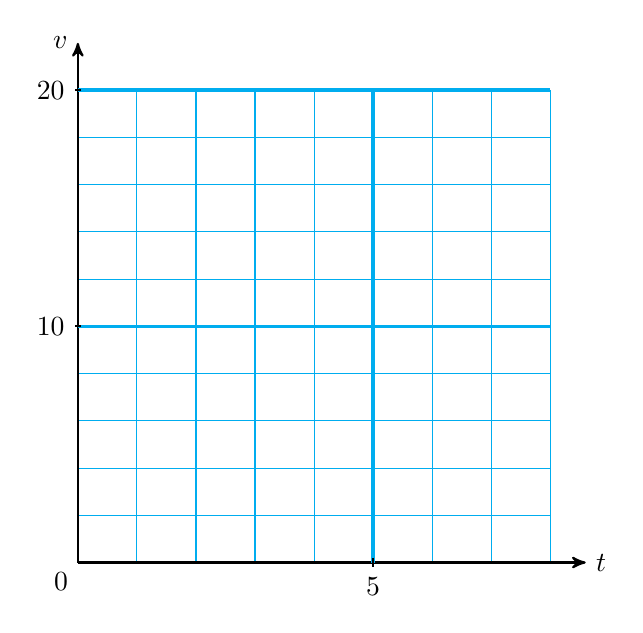
\begin{tikzpicture} [xscale = 0.75, yscale=0.3]
\draw[cyan] (0,0) grid[ystep=2]  (8,20);
\draw[black,thick, ->, >=stealth'] (0,0)--(8.6,0) node[right]{$t$};
\draw[black,thick, ->, >=stealth'] (0,0)--(0,22) node[left]{$v$};
\foreach \x  in  {5} {
 \draw[cyan, very thick] (\x,0) --++(0,20);
 \draw[black, thick] (\x,0.2) --++(0,-.4)  node[below] {\x};
}
\foreach \y in  {10,20} {
 \draw[cyan, very thick] (0, \y) --++(8,0);
 \draw[black, thick] (0.05,\y) --++(-.1,0)  node[left] {\y};
}
\node[below left] at (0,0) {0};
\end{tikzpicture}
\newline


hp-1-1-17aans 

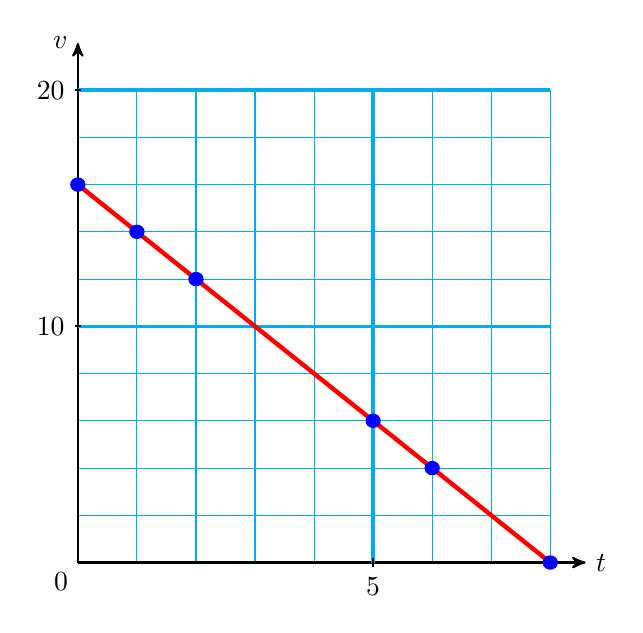
\begin{tikzpicture} [xscale = 0.75, yscale=0.3]
\draw[cyan] (0,0) grid[ystep=2]  (8,20);
\draw[black,thick, ->, >=stealth'] (0,0)--(8.6,0) node[right]{$t$};
\draw[black,thick, ->, >=stealth'] (0,0)--(0,22) node[left]{$v$};
\foreach \x  in  {5} {
 \draw[cyan, very thick] (\x,0) --++(0,20);
 \draw[black, thick] (\x,0.2) --++(0,-.4)  node[below] {\x};
}
\foreach \y in  {10,20} {
 \draw[cyan, very thick] (0, \y) --++(8,0);
 \draw[black, thick] (0.05,\y) --++(-.1,0)  node[left] {\y};
}
\draw[red, ultra thick] (0,16)--(8,0);
\foreach \x [evaluate=\x as \y using int( 16-2*\x )] in  {0,1,2,5,6,8} {
 \filldraw[blue] (\x,\y) ellipse (1.2mm and 2.8mm);
}
\node[below left] at (0,0) {0};
\end{tikzpicture}
\newline


hp-1-1-17b grid

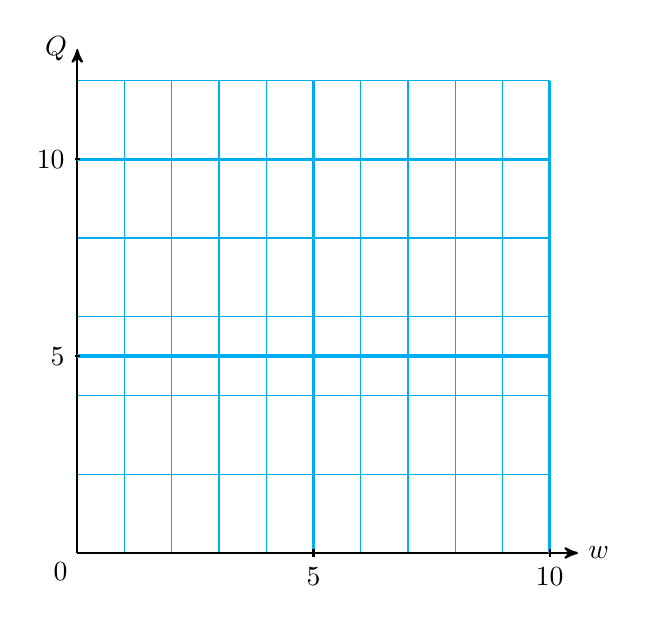
\begin{tikzpicture} [xscale = 0.6, yscale=0.5]
\draw[cyan] (0,0) grid[ystep=2]  (10,12);
\draw[black,thick, ->, >=stealth'] (0,0)--(10.6,0) node[right]{$w$};
\draw[black,thick, ->, >=stealth'] (0,0)--(0,12.8) node[left]{$Q$};
\foreach \x  in  {5,10} {
 \draw[cyan, very thick] (\x,0) --++(0,12);
 \draw[black, thick] (\x,0.1) --++(0,-.2)  node[below] {\x};
}
\foreach \y in  {5,10} {
 \draw[cyan, very thick] (0, \y) --++(10,0);
 \draw[black, thick] (0.05,\y) --++(-.1,0)  node[left] {\y};
}
\node[below left] at (0,0) {0};
\end{tikzpicture}
\newline


hp-1-1-17bans 

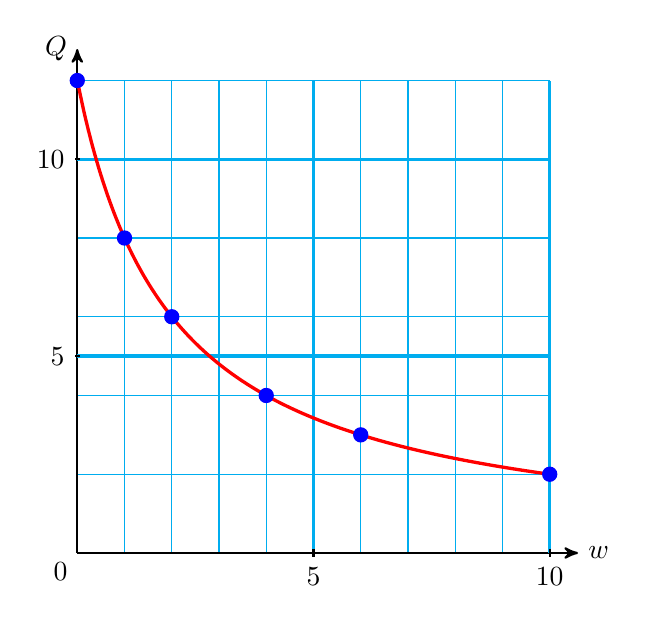
\begin{tikzpicture} [xscale = 0.6, yscale=0.5]
\draw[cyan] (0,0) grid[ystep=2]  (10,12);
\draw[black,thick, ->, >=stealth'] (0,0)--(10.6,0) node[right]{$w$};
\draw[black,thick, ->, >=stealth'] (0,0)--(0,12.8) node[left]{$Q$};
\foreach \x  in  {5,10} {
 \draw[cyan, very thick] (\x,0) --++(0,12);
 \draw[black, thick] (\x,0.1) --++(0,-.2)  node[below] {\x};
}
\foreach \y in  {5,10} {
 \draw[cyan, very thick] (0, \y) --++(10,0);
 \draw[black, thick] (0.05,\y) --++(-.1,0)  node[left] {\y};
}
\draw[samples=65,domain=0:10,smooth,variable=\x,red,very thick] plot ({\x},{24/(\x+2)});
\foreach \x [evaluate=\x as \y using int( 24/(\x+2) )] in  {0,1,2,4,6,10} {
 \filldraw[blue] (\x,\y) ellipse (1.5mm and 1.8mm);
}
\node[below left] at (0,0) {0};
\end{tikzpicture}
\newline


hp-1-1-18 grid and line

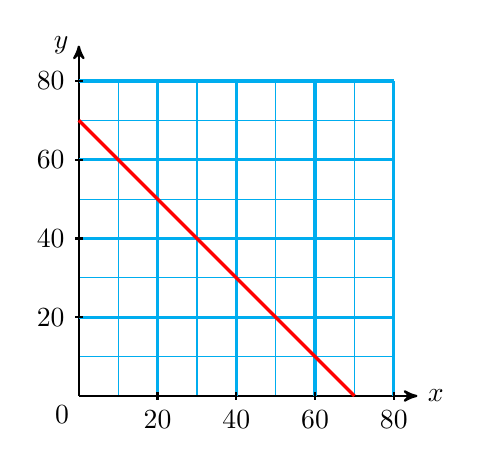
\begin{tikzpicture} [scale=0.05]
\draw[cyan] (0,0) grid[step=10]  (80,80);
\draw[black,thick, ->, >=stealth'] (0,0)--(86,0) node[right]{$x$};
\draw[black,thick, ->, >=stealth'] (0,0)--(0,89) node[left]{$y$};
\foreach \x  in  {20,40,60,80} {
 \draw[cyan, very thick] (\x,0) --++(0,80);
 \draw[black, thick] (\x,1) --++(0,-2)  node[below] {\x};
 \draw[cyan, very thick] (0,\x) --++(80,0);
 \draw[black, thick] (1,\x) --++(-2,0)  node[left] {\x};
}
\draw[red,very thick] (0,70)--(70,0);
\node[below left] at (0,0) {0};
\end{tikzpicture}
\newline


hp-1-1-19 grid

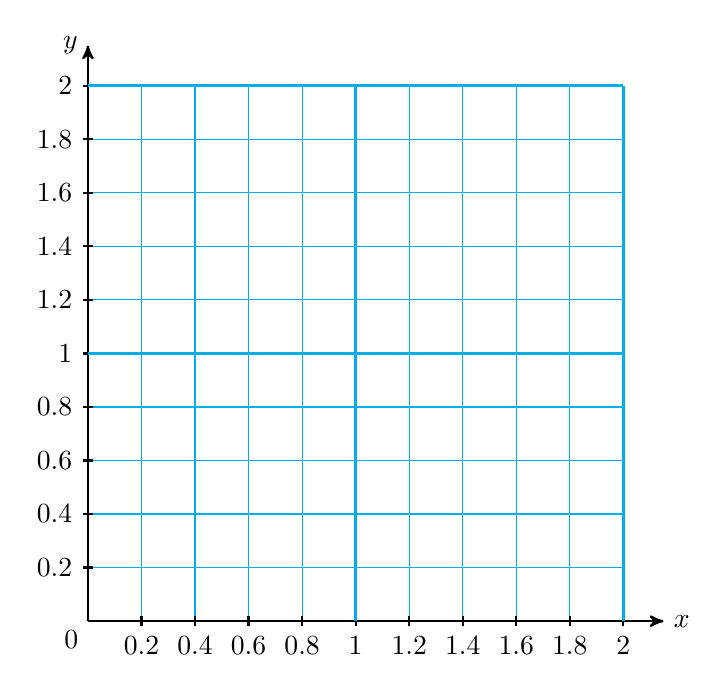
\begin{tikzpicture} [scale=3.4]
\draw[cyan] (0,0) grid[step=1/5]  (2,2);
\draw[black,thick, ->, >=stealth'] (0,0)--(2.15,0) node[right]{$x$};
\draw[black,thick, ->, >=stealth'] (0,0)--(0,2.15) node[left]{$y$};
\foreach \x  in  {0.2, 0.4, 0.6, 0.8,1,1.2,1.4,1.6,1.8, 2} {
 \draw[black, thick] (\x,.02) --++(0,-.04)  node[below] {\x};
 \draw[black, thick] (.02,\x) --++(-.04,0)  node[left] {\x};
}
 \draw[cyan, very thick] (1,0) --++(0,2);
 \draw[cyan, very thick] (0,1) --++(2,0);
 \draw[cyan, very thick] (2,0) --++(0,2);
 \draw[cyan, very thick] (0,2) --++(2,0);
\node[below left] at (0,0) {0};
\end{tikzpicture}
\newline


hp-1-1-19ans line and points

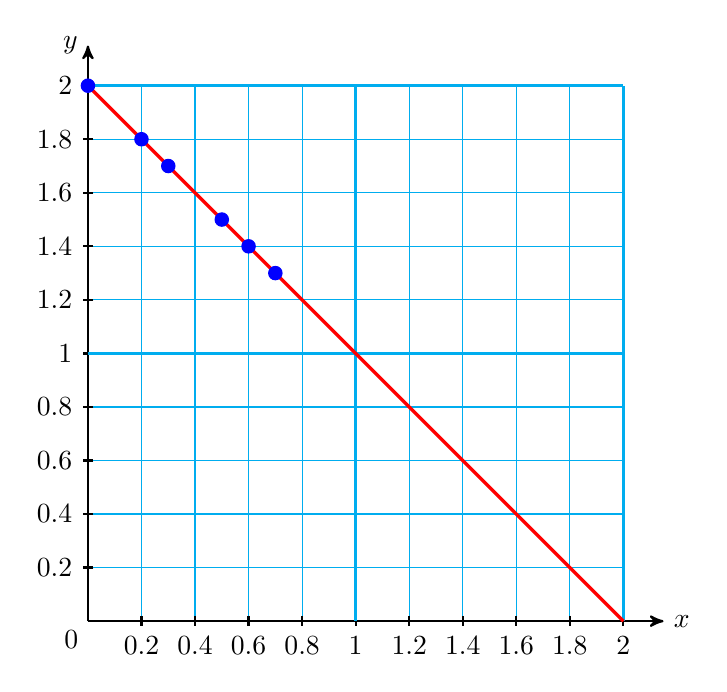
\begin{tikzpicture} [scale=3.4]
\draw[cyan] (0,0) grid[step=1/5]  (2,2);
\draw[black,thick, ->, >=stealth'] (0,0)--(2.15,0) node[right]{$x$};
\draw[black,thick, ->, >=stealth'] (0,0)--(0,2.15) node[left]{$y$};
\foreach \x  in  {0.2, 0.4, 0.6, 0.8,1,1.2,1.4,1.6,1.8, 2} {
 \draw[black, thick] (\x,.02) --++(0,-.04)  node[below] {\x};
 \draw[black, thick] (.02,\x) --++(-.04,0)  node[left] {\x};
}
 \draw[cyan, very thick] (1,0) --++(0,2);
 \draw[cyan, very thick] (0,1) --++(2,0);
 \draw[cyan, very thick] (2,0) --++(0,2);
 \draw[cyan, very thick] (0,2) --++(2,0);
\node[below left] at (0,0) {0};
\draw[red,very thick] (0,2)--(2,0);
\foreach \x [evaluate=\x as \y using ( 2-\x) )] in  {0,0.2,0.3,0.5,0.6,0.7} {
 \filldraw[blue] (\x,\y) circle (.25mm);
}
\end{tikzpicture}
\newline


hp-1-1-20 grid

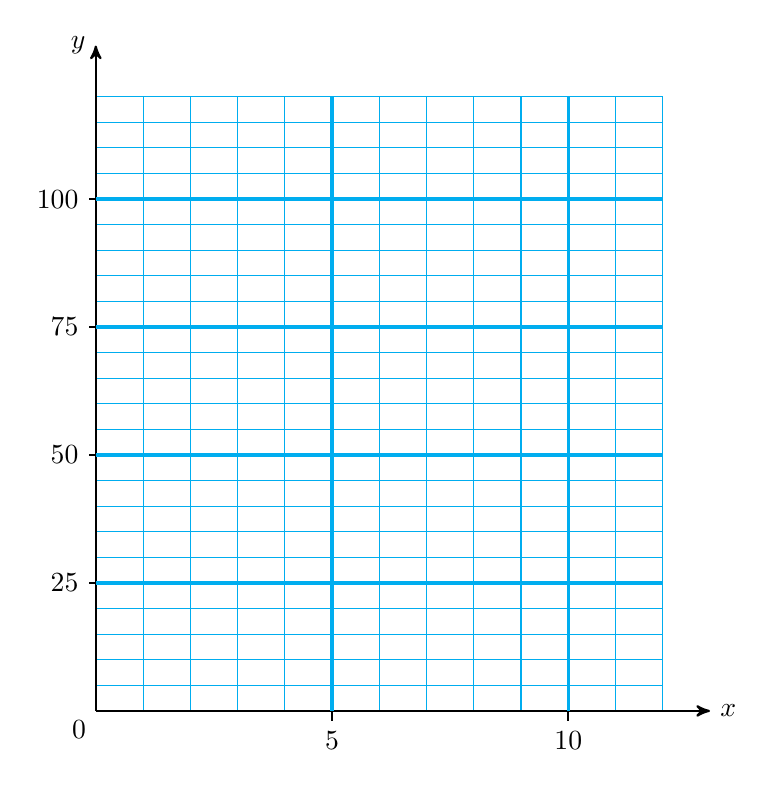
\begin{tikzpicture} [xscale=0.6, yscale=.065]
\draw[cyan] (0,0) grid[ystep=5]  (12,120);
\draw[black,thick, ->, >=stealth'] (0,0)--(13,0) node[right]{$x$};
\draw[black,thick, ->, >=stealth'] (0,0)--(0,130) node[left]{$y$};
\foreach \x  in  {5,10} {
 \draw[black, thick] (\x,2) --++(0,-4)  node[below] {\x};
 \draw[cyan, very thick] (\x,0) --++(0,120);
}
\foreach \y  in  {25,50,75,100} {
 \draw[black, thick] (.15,\y) --++(-.3,0)  node[left] {\y};
 \draw[cyan, very thick] (0,\y) --++(12,0);
}
\node[below left] at (0,0) {0};
\end{tikzpicture}
\newline



\section{Chap 1 Section 2}

Sums  fig-1-2-1

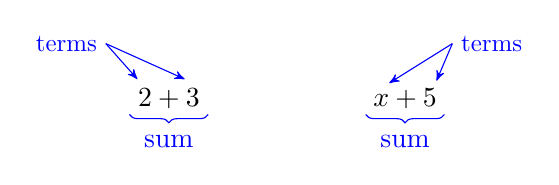
\begin{tikzpicture} 
\coordinate (O) at (0,0);
\coordinate (A) at (-0.8,0.7);
\coordinate (Aa) at (-0.4,.25);
\coordinate (Ab) at (0.2,.25);
\coordinate (B) at (-.5,-.2);
\node at (O) {$2+3$};
\draw[blue, <-, >=stealth'] (Ab)--(A) node[left, scale=.9]{terms};
\draw[blue, <-, >=stealth'] (Aa)--(A);
\draw [blue,decorate,decoration={brace,amplitude=3pt}] (.5,-0.2)--(B)  node [below,midway,yshift=-4pt] {sum};
\coordinate (P) at (3,0);
\coordinate (C) at (3.6,0.7);
\coordinate (Ca) at (2.8,.2);
\coordinate (Cb) at (3.4,.23);
\coordinate (D) at (2.5,-.2);
\node at (P) {$x+5$};
\draw[blue, <-, >=stealth'] (Cb)--(C) node[right, scale=.9]{terms};
\draw[blue, <-, >=stealth'] (Ca)--(C);
\draw [blue,decorate,decoration={brace,amplitude=3pt}] (3.5,-0.2)--(D)  node [below,midway,yshift=-4pt] {sum};
\end{tikzpicture}
\newline


Products  fig-1-2-2

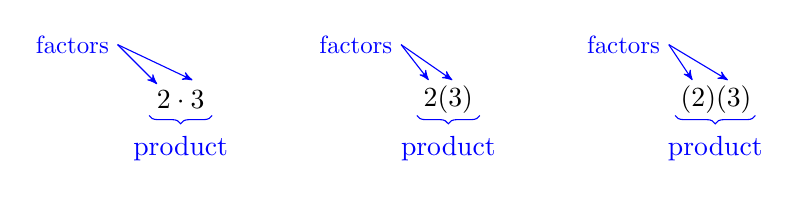
\begin{tikzpicture} 
\coordinate (O) at (0,0);
\coordinate (A) at (-0.8,0.7);
\coordinate (Aa) at (-0.3,.2);
\coordinate (Ab) at (0.15,.25);
\coordinate (B) at (-.4,-.2);
\node at (O) {$2\cdot3$};
\draw[blue, <-, >=stealth'] (Ab)--(A) node[left, scale=.9]{factors};
\draw[blue, <-, >=stealth'] (Aa)--(A);
\draw [blue,decorate,decoration={brace,amplitude=3pt}] (.4,-0.2)--(B)  node [below,midway,yshift=-4pt] {product};
\coordinate (P) at (3.4,0);
\coordinate (C) at (2.8,0.7);
\coordinate (Ca) at (3.15,.25);
\coordinate (Cb) at (3.45,.25);
\coordinate (D) at (3,-.2);
\node at (P) {$2(3)$};
\draw[blue, <-, >=stealth'] (Cb)--(C) node[left, scale=.9]{factors};
\draw[blue, <-, >=stealth'] (Ca)--(C);
\draw [blue,decorate,decoration={brace,amplitude=3pt}] (3.8,-0.2)--(D)  node [below,midway,yshift=-4pt] {product};
\coordinate (Q) at (6.8,0);
\coordinate (E) at (6.2,0.7);
\coordinate (Ea) at (6.5,.25);
\coordinate (Eb) at (6.95,.25);
\coordinate (F) at (6.28,-.2);
\node at (Q) {$(2)(3)$};
\draw[blue, <-, >=stealth'] (Eb)--(E) node[left, scale=.9]{factors};
\draw[blue, <-, >=stealth'] (Ea)--(E);
\draw [blue,decorate,decoration={brace,amplitude=3pt}] (7.3,-0.2)--(F)  node [below,midway,yshift=-4pt] {product};
\end{tikzpicture}
\newline



Differences  fig-1-2-3

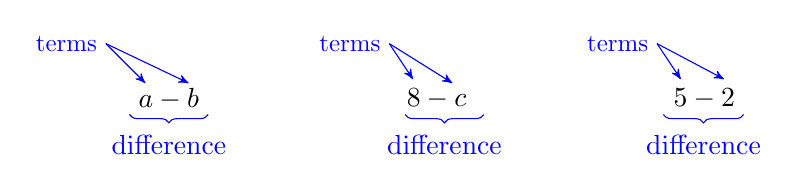
\begin{tikzpicture} 
\coordinate (O) at (0,0);
\coordinate (A) at (-0.8,0.7);
\coordinate (Aa) at (-0.3,.2);
\coordinate (Ab) at (0.25,.2);
\coordinate (B) at (-.5,-.2);
\node at (O) {$a-b$};
\draw[blue, <-, >=stealth'] (Ab)--(A) node[left, scale=.9]{terms};
\draw[blue, <-, >=stealth'] (Aa)--(A);
\draw [blue,decorate,decoration={brace,amplitude=3pt}] (.5,-0.2)--(B)  node [below,midway,yshift=-4pt] {difference};
\coordinate (P) at (3.4,0);
\coordinate (C) at (2.8,0.7);
\coordinate (Ca) at (3.1,.25);
\coordinate (Cb) at (3.6,.2);
\coordinate (D) at (3,-.2);
\node at (P) {$8-c$};
\draw[blue, <-, >=stealth'] (Cb)--(C) node[left, scale=.9]{terms};
\draw[blue, <-, >=stealth'] (Ca)--(C);
\draw [blue,decorate,decoration={brace,amplitude=3pt}] (4.,-0.2)--(D)  node [below,midway,yshift=-4pt] {difference};
\coordinate (Q) at (6.8,0);
\coordinate (E) at (6.2,0.7);
\coordinate (Ea) at (6.5,.25);
\coordinate (Eb) at (7.05,.25);
\coordinate (F) at (6.28,-.2);
\node at (Q) {$5-2$};
\draw[blue, <-, >=stealth'] (Eb)--(E) node[left, scale=.9]{terms};
\draw[blue, <-, >=stealth'] (Ea)--(E);
\draw [blue,decorate,decoration={brace,amplitude=3pt}] (7.3,-0.2)--(F)  node [below,midway,yshift=-4pt] {difference};
\end{tikzpicture}
\newline


Quotients  fig-1-2-4

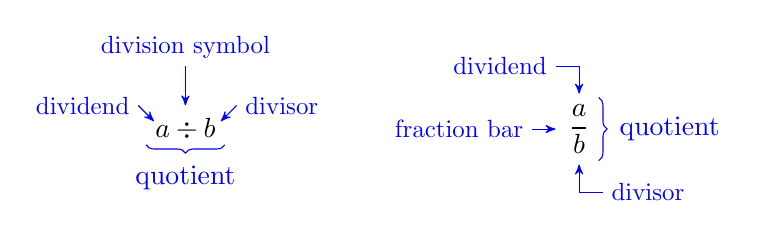
\begin{tikzpicture} 
\coordinate (O) at (0,0);
\coordinate (A) at (0,0.8);
\coordinate (B) at (-.6,0.3);
\coordinate (B2) at (.65,0.3);
\coordinate (C) at (-.5,-0.2);
\node at (O) {$a\div b$};
\draw[blue, <-, >=stealth'] (A)++(0,-.5)--(A) node[above, yshift=-.3, scale=.9]{division symbol};
\draw[blue, <-, >=stealth'] (B)++(.2,-0.2)--(B) node[left, scale=.9] {dividend};;
\draw[blue, <-, >=stealth'] (B2)++(-.2,-0.2)--(B2) node[right, scale=.9] {divisor};;
\draw [blue,decorate,decoration={brace,amplitude=3pt}] (C)++(1,0)--(C)  node [below,midway,yshift=-4pt] {quotient};
\coordinate (P) at (5,0);
\coordinate (D) at (5,0.8);
\coordinate (E) at (4.4,0);
\coordinate (E2) at (5.25,0);
\coordinate (F) at (5,-.8);
\node at (P) {$\displaystyle\frac{a}{b}$};
\draw[blue, <-, >=stealth'] (D)++(0,-.35)--(D)--++(-0.3,0) node[left, scale=.9]{dividend};
\draw[blue, <-, >=stealth'] (E)++(.3,0)--(E) node[left, scale=.9] {fraction bar};;
\draw[blue, <-, >=stealth'] (F)++(0,.35)--(F)--++(0.3,0) node[right, scale=.9] {divisor};;
\draw [blue,decorate,decoration={brace,amplitude=3pt}] (E2)++(0,0.4)--++(0,-0.8)  node [right,midway,xshift=4pt] {quotient};
\end{tikzpicture}
\newline


Squares sw-1-2-7

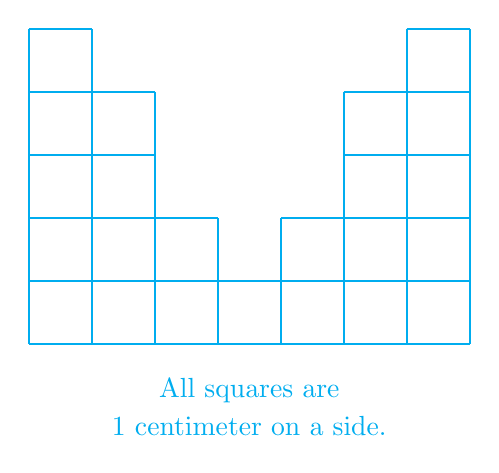
\begin{tikzpicture} [scale=0.8]
\draw[cyan, thick] (-3,0) grid (-2,5);
\draw[cyan, thick] (-2,0) grid (-1,4);
\draw[cyan, thick] (-1,0) grid (0,2);
\draw[cyan, thick] (0,0) grid (1,1);
\draw[cyan, thick] (3,0) grid (4,5);
\draw[cyan, thick] (2,0) grid (3,4);
\draw[cyan, thick] (1,0) grid (2,2);
\node[below,text=cyan] at (0.5,-0.4){All squares are};
\node[below,text=cyan] at (0.5,-1){1 centimeter on a side.};
\end{tikzpicture}
\newline


polygonal sw-1-2-8

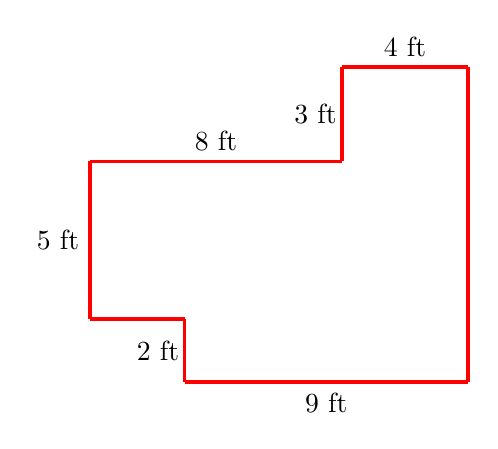
\begin{tikzpicture} [scale=0.4]
\draw[red,very thick] (0,0)--++(0,5) node[left, midway, text=black]{5 ft};
\draw[red,very thick] (0,5)--++(8,0) node[above, midway, text=black]{8 ft};
\draw[red,very thick] (8,5)--++(0,3) node[left, midway, xshift=2, text=black]{3 ft};
\draw[red,very thick] (8,8)--++(4,0) node[above, midway, text=black]{4 ft};
\draw[red,very thick] (0,0)--++(3,0);
\draw[red,very thick] (3,0)--++(0,-2) node[left, midway, xshift=2, text=black]{2 ft};
\draw[red,very thick] (3,-2)--++(9,0) node[below, midway, text=black]{9 ft};
\draw[red, very thick](12,8)--++(0,-10);
\end{tikzpicture}
\newline




\section{Chap 1 Section 3}

Example fig-1-3-ex1

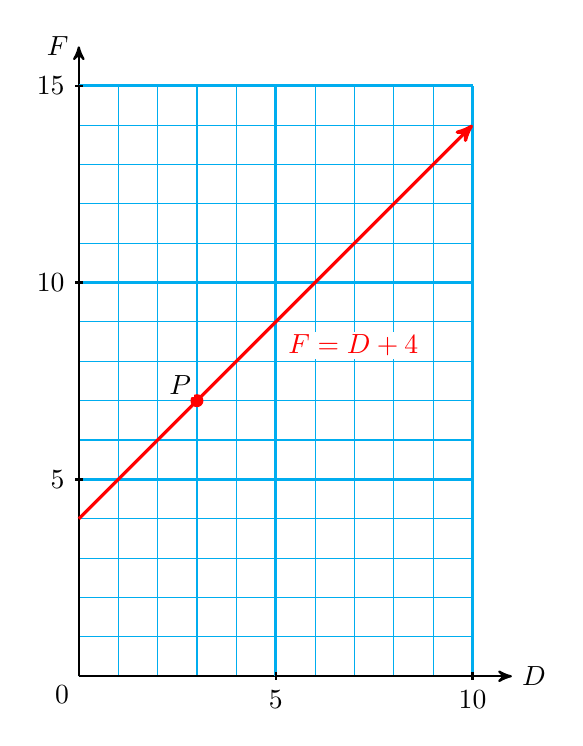
\begin{tikzpicture} [scale=0.5]
\draw[cyan] (0,0) grid (10,15);
\draw[black,thick, ->, >=stealth'] (0,0)--(11,0) node[right]{$D$};
\draw[black,thick, ->, >=stealth'] (0,0)--(0,16) node[left]{$F$};
\foreach \x in  {5,10} {
 \draw[cyan, very thick] (\x,0) --++(0,15);
 \draw[black, thick] (\x,.1) --++(0,-.2)  node[below]   {\x};
}
\foreach \y in  {5,10,15} {
 \draw[cyan, very thick] (0,\y) --++(10,0);
 \draw[black, thick] (.1,\y) --++(-.2,0)  node[left]   {\y};
}
\filldraw[red] (3,7) circle (0.15cm) node[above left, xshift=-1, yshift=1, fill=white, inner sep = 1, text=black] {$P$};
\draw [red, very thick, ->, >=stealth']  (0,4) -- (10,14) node[below right, xshift=3, yshift=-3, midway, fill=white, inner sep=1] {$F=D+4$};
\node[below left] at (0,0) {0};
\end{tikzpicture}
\newline


fig-1-3-ex2

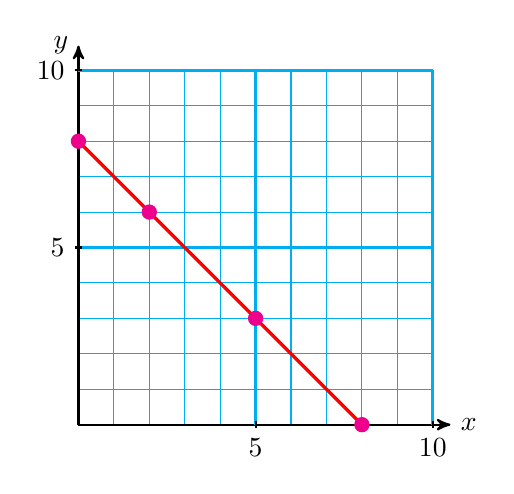
\begin{tikzpicture} [scale=0.45]
\draw[cyan] (0,0) grid (10,10);
\draw[black,thick, ->, >=stealth'] (0,0)--(10.5,0) node[right]{$x$};
\draw[black,thick, ->, >=stealth'] (0,0)--(0,10.7) node[left]{$y$};
\foreach \x in  {5,10} {
 \draw[cyan, very thick] (\x,0) --++(0,10);
 \draw[black, thick] (\x,.1) --++(0,-.2)  node[below]   {\x};
}
\foreach \y in  {5,10} {
 \draw[cyan, very thick] (0,\y) --++(10,0);
 \draw[black, thick] (.1,\y) --++(-.2,0)  node[left]   {\y};
}
\draw [red, very thick]  (0,8) -- (8,0);
\filldraw[magenta] (0,8) circle (0.2cm);
\filldraw[magenta] (8,0) circle (0.2cm);
\filldraw[magenta] (2,6) circle (0.2cm);
\filldraw[magenta] (5,3) circle (0.2cm);
\end{tikzpicture}
\newline


fig-1-3-ex3

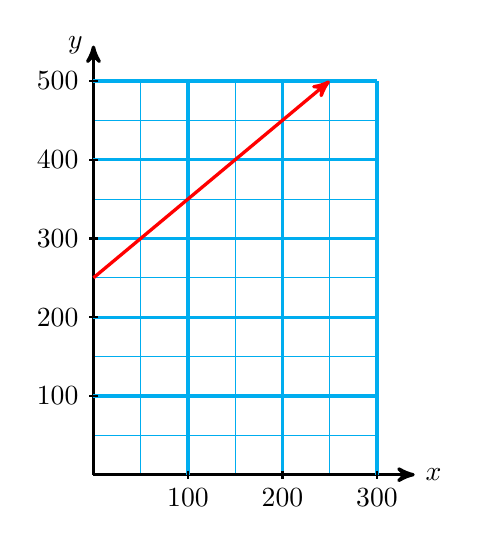
\begin{tikzpicture} [xscale =.6, yscale=0.5]
\draw[cyan] (0,0) grid (6,10);
\draw[black,very thick, ->, >=stealth'] (0,0)--(6.8,0) node[right]{$x$};
\draw[black,very thick, ->, >=stealth'] (0,0)--(0,10.9) node[left]{$y$};
\foreach \x [evaluate=\x as \xi using int(50*\x)] in  {2,4,6} {
 \draw[cyan, very thick] (\x,0) --++(0,10);
 \draw[black, thick] (\x,.1) --++(0,-.2)  node[below]   {\xi};
}
\foreach \y [evaluate=\y as \yi using int(50*\y)] in  {2,4,6,8,10} {
 \draw[cyan, very thick] (0,\y) --++(6,0);
 \draw[black, thick] (.1,\y) --++(-.2,0)  node[left]   {\yi};
}
\draw [red, very thick, ->, >=stealth']  (0,5) -- (5,10);
\end{tikzpicture}
\newline


Caution fig-1-3-1

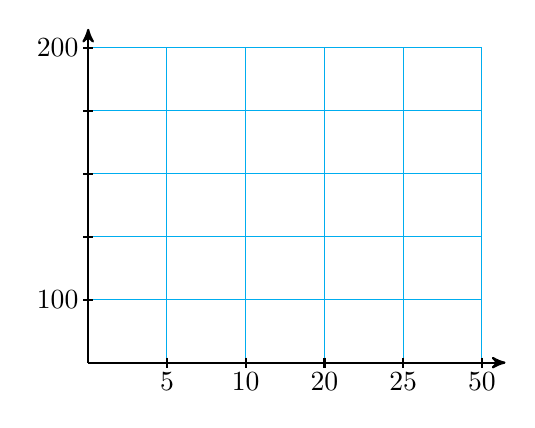
\begin{tikzpicture} [yscale=0.8]
\draw[cyan] (0,0) grid (5,5);
\draw[black,thick, ->, >=stealth'] (0,0)--(5.3,0);
\draw[black,thick, ->, >=stealth'] (0,0)--(0,5.3);
\foreach \x in  {1,2,3,4,5} {
 \draw[black, thick] (\x,.08) --++(0,-.16);
}
\foreach \y in  {1,2,3,4,5} {
 \draw[black, thick] (.06,\y) --++(-.12,0);
}
\node[below] at (1,0) {5};
\node[below] at (2,0) {10};
\node[below] at (3,0) {20};
\node[below] at (4,0) {25};
\node[below] at (5,0) {50};
\node[left] at (0,1) {100};
\node[left] at (0,5) {200};
\end{tikzpicture}
\newline


Example 5 fig-1-3-ex5

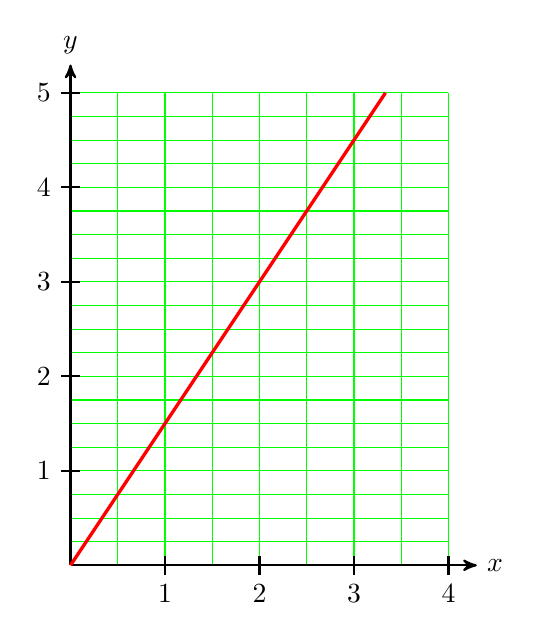
\begin{tikzpicture} [scale=1.2]
\draw[green] (0,0) grid[xstep=1/2, ystep=1/4] (4,5);
\draw[black,thick, ->, >=stealth'] (0,0)--(4.3,0) node[right]{$x$};
\draw[black,thick, ->, >=stealth'] (0,0)--(0,5.3) node[above]{$y$};
\foreach \x in  {1,2,3,4} {
 \draw[black, thick] (\x,.1) --++(0,-.2)  node[below]   {\x};
}
\foreach \y in  {1,2,3,4,5} {
 \draw[black, thick] (.1,\y) --++(-.2,0)  node[left]   {\y};
}
\draw [red, very thick]  (0,0) -- (10/3,5);
\end{tikzpicture}
\newline

Example 5 fig-1-3-ex5ans

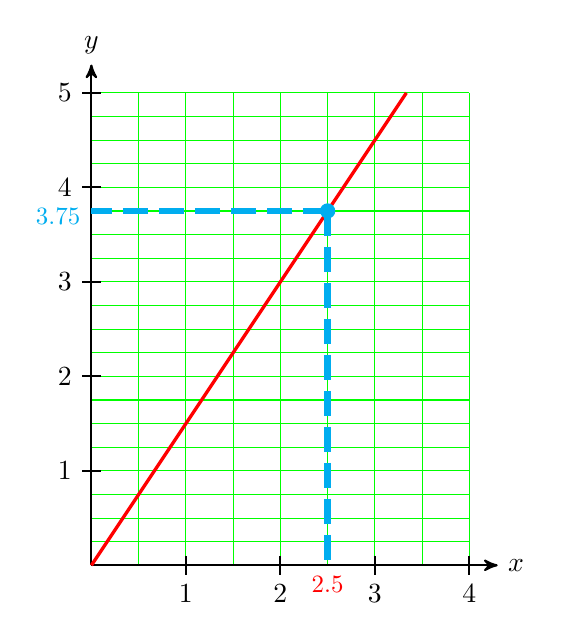
\begin{tikzpicture} [scale=1.2]
\draw[green] (0,0) grid[xstep=1/2, ystep=1/4] (4,5);
\draw[black,thick, ->, >=stealth'] (0,0)--(4.3,0) node[right]{$x$};
\draw[black,thick, ->, >=stealth'] (0,0)--(0,5.3) node[above]{$y$};
\foreach \x in  {1,2,3,4} {
 \draw[black, thick] (\x,.1) --++(0,-.2)  node[below]   {\x};
}
\foreach \y in  {1,2,3,4,5} {
 \draw[black, thick] (.1,\y) --++(-.2,0)  node[left]   {\y};
}
\draw [red, very thick]  (0,0) -- (10/3,5);
\draw[line width=0.8mm, cyan, dashed, dash pattern=on 9pt off 4pt] (2.5,3.75) -- (2.5,0) node[below, text=red, scale=0.9] {2.5};
\draw[line width=0.8mm, cyan, dashed, dash pattern=on 9pt off 4pt] (2.5,3.75) -- (0,3.75) node[left, yshift=-2pt, text=cyan, scale=0.9] {3.75};
\draw[cyan, fill=cyan] (2.5,3.75) circle(.75mm);
\end{tikzpicture}
\newline

grid hp-1-3-7

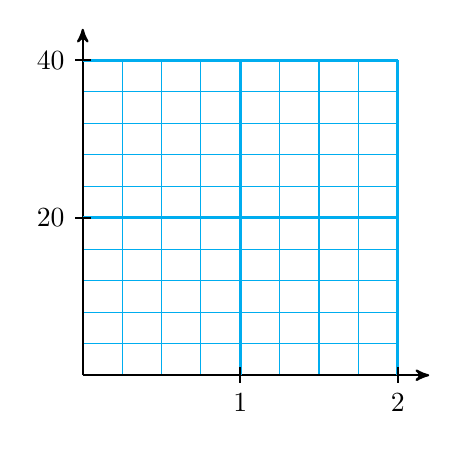
\begin{tikzpicture} [scale=2]
\draw[cyan] (0,0) grid[xstep=1/4, ystep=1/5] (2,2);
\draw[black,thick, ->, >=stealth'] (0,0)--(2.2,0);
\draw[black,thick, ->, >=stealth'] (0,0)--(0,2.2);
\foreach \x  in  {1,2} {
 \draw[cyan, very thick] (\x,.0) --++(0,2);
 \draw[black, thick] (\x,.05) --++(0,-.1)  node[below] {\x};
}
\foreach \y [evaluate=\y as \yi using int( 20* \y )]  in  {1,2} {
 \draw[cyan, very thick] (0,\y) --++(2,0);
 \draw[black, thick] (.05,\y) --++(-.1,0)  node[left]   {\yi};
}
\end{tikzpicture}
\newline

grid hp-1-3-8

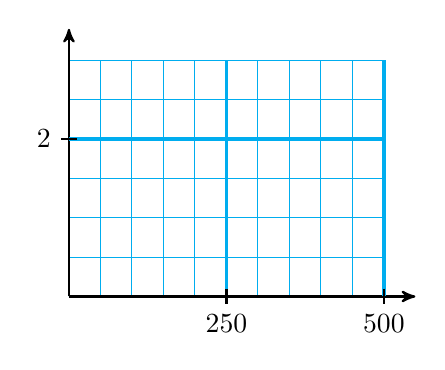
\begin{tikzpicture} [scale=2]
\draw[cyan] (0,0) grid[xstep=1/5, ystep=1/4] (2,3/2);
\draw[black,thick, ->, >=stealth'] (0,0)--(2.2,0);
\draw[black,thick, ->, >=stealth'] (0,0)--(0,1.7);
\foreach \x [evaluate=\x as \xi using int( 250* \x )]  in  {1,2} {
 \draw[cyan, very thick] (\x,.0) --++(0,1.5);
 \draw[black, thick] (\x,.05) --++(0,-.1)  node[below] {\xi};
}
\foreach \y [evaluate=\y as \yi using int( 2* \y )]  in  {1} {
 \draw[cyan, very thick] (0,\y) --++(2,0);
 \draw[black, thick] (.05,\y) --++(-.1,0)  node[left]   {\yi};
}
\end{tikzpicture}
\newline

hp-1-3-9


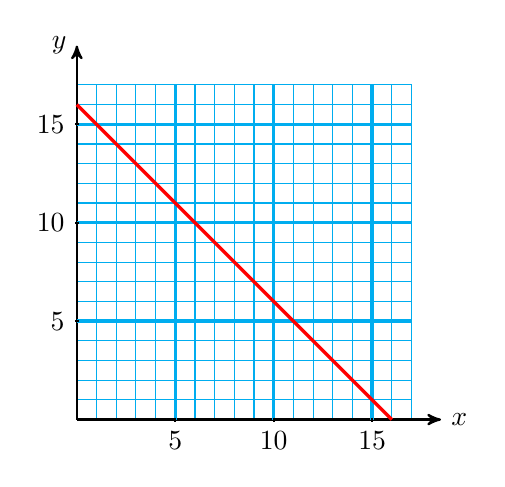
\begin{tikzpicture} [scale=.25]
\draw[cyan] (0,0) grid (17,17);
\draw[black,thick, ->, >=stealth'] (0,0)--(18.5,0) node[right]{$x$};
\draw[black,thick, ->, >=stealth'] (0,0)--(0,19) node[left]{$y$};
\foreach \x  in  {5,10,15} {
 \draw[cyan, very thick] (\x,.0) --++(0,17);
 \draw[black, thick] (\x,.1) --++(0,-.2)  node[below] {\x};
}
\foreach \y in  {5,10,15} {
 \draw[cyan, very thick] (0,\y) --++(17,0);
 \draw[black, thick] (.1,\y) --++(-.2,0)  node[left]   {\y};
}
\draw[red,very thick](0,16)--(16,0);
\end{tikzpicture}
\newline

hp-1-3-10


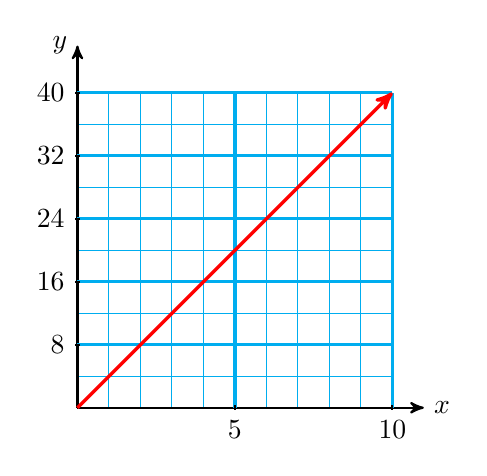
\begin{tikzpicture} [scale=.4]
\draw[cyan] (0,0) grid (10,10);
\draw[black,thick, ->, >=stealth'] (0,0)--(11,0) node[right]{$x$};
\draw[black,thick, ->, >=stealth'] (0,0)--(0,11.5) node[left]{$y$};
\foreach \x  in  {5,10} {
 \draw[cyan, very thick] (\x,.0) --++(0,10);
 \draw[black, thick] (\x,.08) --++(0,-.16)  node[below] {\x};
}
\foreach \y [evaluate=\y as \yi using int( 4* \y )] in  {2,4,...,10} {
 \draw[cyan, very thick] (0,\y) --++(10,0);
 \draw[black, thick] (.08,\y) --++(-.16,0)  node[left]   {\yi};
}
\draw[red,very thick, ->, >=stealth'](0,0)--(10,10);
\end{tikzpicture}
\newline


hp-1-3-11

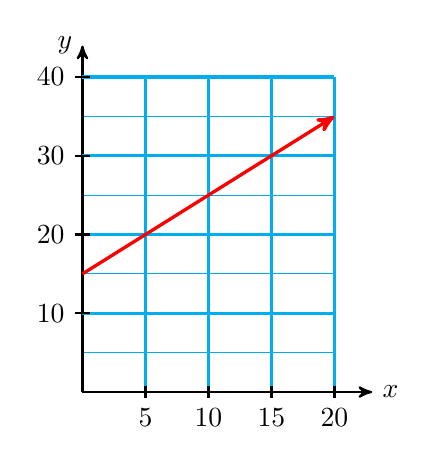
\begin{tikzpicture} [xscale=.16, yscale=.10]
\draw[cyan] (0,0) grid[step=5] (20,40);
\draw[black,thick, ->, >=stealth'] (0,0)--(23,0) node[right]{$x$};
\draw[black,thick, ->, >=stealth'] (0,0)--(0,44) node[left]{$y$};
\foreach \x  in  {5,10,15,20} {
 \draw[cyan, very thick] (\x,.0) --++(0,40);
 \draw[black, thick] (\x,.8) --++(0,-1.6)  node[below] {\x};
}
\foreach \y in  {10,20,30,40} {
 \draw[cyan, very thick] (0,\y) --++(20,0);
 \draw[black, thick] (.6,\y) --++(-1.2,0)  node[left]   {\y};
}
\draw[red,very thick, ->, >=stealth'](0,15)--(20,35);
\end{tikzpicture}
\newline


hp-1-3-12

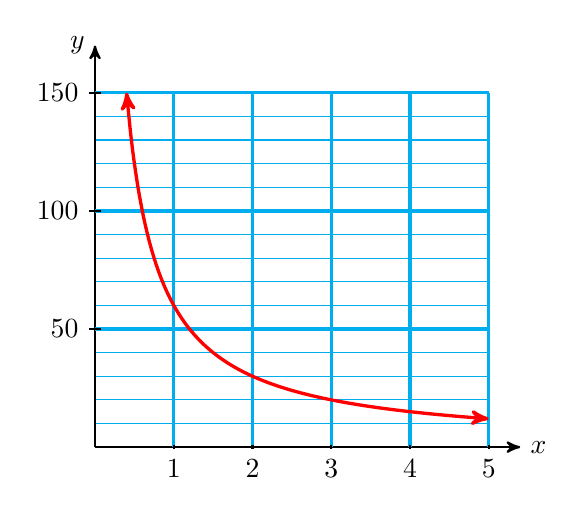
\begin{tikzpicture} [yscale=.03]
\draw[cyan] (0,0) grid[ystep=10] (5,150);
\draw[black,thick, ->, >=stealth'] (0,0)--(5.4,0) node[right]{$x$};
\draw[black,thick, ->, >=stealth'] (0,0)--(0,170) node[left]{$y$};
\foreach \x  in  {1,2,3,4,5} {
 \draw[cyan, very thick] (\x,.0) --++(0,150);
 \draw[black, thick] (\x,1) --++(0,-2)  node[below] {\x};
}
\foreach \y in  {50,100, 150} {
 \draw[cyan, very thick] (0,\y) --++(5,0);
 \draw[black, thick] (.08,\y) --++(-.16,0)  node[left]   {\y};
}
\draw[samples=65,domain=2/5:5,smooth,variable=\x,red,very thick, <->, >=stealth'] plot ({\x},{60/\x)});
\end{tikzpicture}
\newline


hp-1-3-13

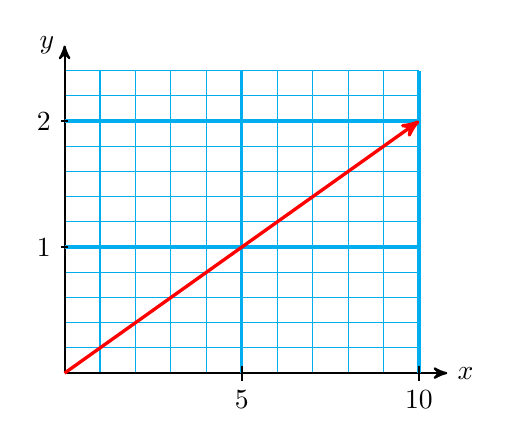
\begin{tikzpicture} [xscale=.45,yscale=1.6]
\draw[cyan] (0,0) grid[ystep=1/5] (10,2.4);
\draw[black,thick, ->, >=stealth'] (0,0)--(10.8,0) node[right]{$x$};
\draw[black,thick, ->, >=stealth'] (0,0)--(0,2.6) node[left]{$y$};
\foreach \x  in  {5,10} {
 \draw[cyan, very thick] (\x,.0) --++(0,2.4);
 \draw[black, thick] (\x,.06) --++(0,-.12)  node[below] {\x};
}
\foreach \y in  {1,2} {
 \draw[cyan, very thick] (0,\y) --++(10,0);
 \draw[black, thick] (.1,\y) --++(-.2,0)  node[left]   {\y};
}
\draw[red,very thick, ->, >=stealth'] (0,0)--(10,2);
\end{tikzpicture}
\newline


hp-1-3-14

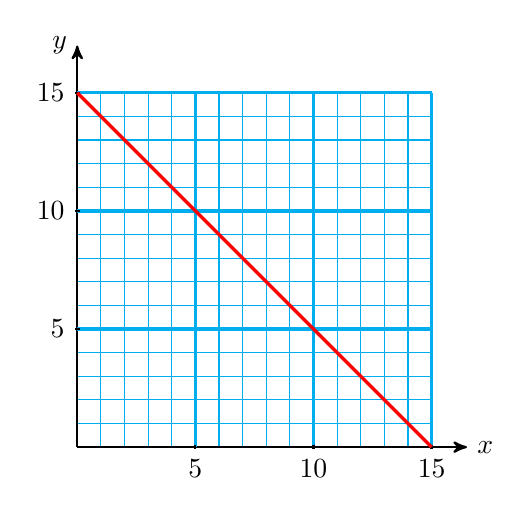
\begin{tikzpicture} [scale=.3]
\draw[cyan] (0,0) grid (15,15);
\draw[black,thick, ->, >=stealth'] (0,0)--(16.5,0) node[right]{$x$};
\draw[black,thick, ->, >=stealth'] (0,0)--(0,17) node[left]{$y$};
\foreach \x  in  {5,10,15} {
 \draw[cyan, very thick] (\x,.0) --++(0,15);
 \draw[black, thick] (\x,.1) --++(0,-.2)  node[below] {\x};
}
\foreach \y in  {5,10,15} {
 \draw[cyan, very thick] (0,\y) --++(15,0);
 \draw[black, thick] (.1,\y) --++(-.2,0)  node[left]   {\y};
}
\draw[red,very thick](0,15)--(15,0);
\end{tikzpicture}
\newline


hp-1-3-15

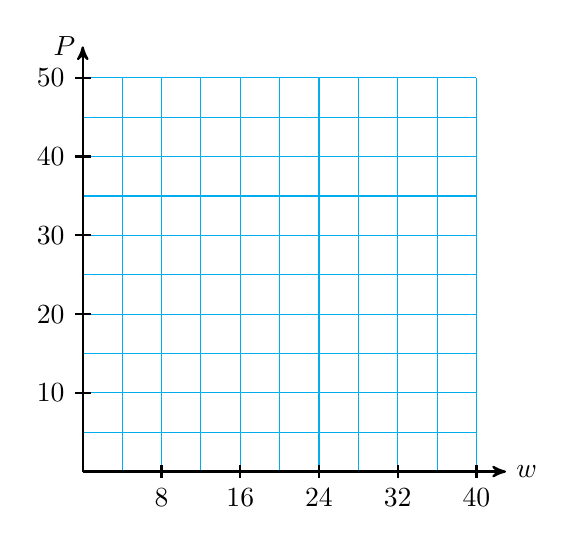
\begin{tikzpicture} [xscale=.125, yscale=.1]
\draw[cyan] (0,0) grid[xstep=4, ystep=5] (40,50);
\draw[black,thick, ->, >=stealth'] (0,0)--(43,0) node[right]{$w$};
\draw[black,thick, ->, >=stealth'] (0,0)--(0,54) node[left, xshift=1]{$P$};
\foreach \x  in  {8,16,...,40} {
 \draw[black, thick] (\x,0.8) --++(0,-1.6)  node[below] {\x};
}
\foreach \y in  {10, 20, 30, 40,50} {
 \draw[black, thick] (.8,\y) --++(-1.6,0)  node[left]   {\y};
}
\end{tikzpicture}
\newline


hp-1-3-15ans

\begin{tikzpicture} [xscale=.125, yscale=.1]
\draw[cyan] (0,0) grid[xstep=4, ystep=5] (40,50);
\draw[black,thick, ->, >=stealth'] (0,0)--(43,0) node[right]{$w$};
\draw[black,thick, ->, >=stealth'] (0,0)--(0,54) node[left, xshift=1]{$P$};
\foreach \x  in  {8,16,...,40} {
 \draw[black, thick] (\x,0.8) --++(0,-1.6)  node[below] {\x};
}
\foreach \y in  {10, 20, 30, 40,50} {
 \draw[black, thick] (.8,\y) --++(-1.6,0)  node[left]   {\y};
}
\draw[red,ultra thick,->,>=stealth'] (0,0)--(40,50);
\filldraw[blue] (12,15) ellipse (8mm and 10mm);
\filldraw[blue] (16,20) ellipse (8mm and 10mm);
\filldraw[blue] (20,25) ellipse (8mm and 10mm);
\filldraw[blue] (30,37.5) ellipse (8mm and 10mm);
\filldraw[blue] (36,45) ellipse (8mm and 10mm);
\filldraw[blue] (40,50) ellipse (8mm and 10mm);
\end{tikzpicture}
\newline


hp-1-3-16 grid

\begin{tikzpicture} [scale=.5]
\draw[cyan] (0,0) grid (10,10);
\draw[black,thick, ->, >=stealth'] (0,0)--(10.5,0) node[right]{$L$};
\draw[black,thick, ->, >=stealth'] (0,0)--(0,10.5) node[left, xshift=1]{$D$};
\foreach \x  in  {1,2,...,10} {
 \draw[black, thick] (\x,0.09) --++(0,-.18);
}
\foreach \y in  {1,2,...,10} {
 \draw[black, thick] (.09,\y) --++(-.18,0);
}
\end{tikzpicture}
\newline


hp-1-3-17 grid

\begin{tikzpicture} [scale=.5]
\draw[cyan] (0,0) grid (10,10);
\draw[black,thick, ->, >=stealth'] (0,0)--(10.5,0) node[right]{$m$};
\draw[black,thick, ->, >=stealth'] (0,0)--(0,10.5) node[left, xshift=1]{$S$};
\foreach \x  in  {1,2,...,10} {
 \draw[black, thick] (\x,0.09) --++(0,-.18);
}
\foreach \y in  {1,2,...,10} {
 \draw[black, thick] (.09,\y) --++(-.18,0);
}
\end{tikzpicture}
\newline


hp-1-3-17ans hyperbola

\begin{tikzpicture} [scale=.5]
\draw[cyan] (0,0) grid (10,10);
\draw[black,thick, ->, >=stealth'] (0,0)--(10.5,0) node[right]{$m$};
\draw[black,thick, ->, >=stealth'] (0,0)--(0,10.5) node[above]{$S$};
\foreach \x [evaluate=\x as \xi using int( 10* \x )] in  {2,4,...,10} {
 \draw[black, thick] (\x,0.09) --++(0,-.18) node[below]{\xi};
}
\foreach \y [evaluate=\y as \yi using int( 40* \y )] in  {5,10} {
 \draw[black, thick] (.09,\y) --++(-.18,0) node[left]{\yi};
}
\draw[samples=65,domain=.9:10,smooth,variable=\x,red,very thick, <->, >=stealth'] plot ({\x},{9/\x)});
\filldraw[blue](2,4.5) circle (.15cm);
\filldraw[blue](4,2.25) circle (.15cm);
\filldraw[blue](6,1.5) circle (.15cm);
\filldraw[blue](10,0.9) circle (.15cm);
\end{tikzpicture}
\newline


hp-1-3-18

\begin{tikzpicture} [scale=.04]
\draw[cyan] (0,0) grid[step=10] (150,150);
\draw[black,thick, ->, >=stealth'] (0,0)--(165,0) node[right]{$p$};
\draw[black,thick, ->, >=stealth'] (0,0)--(0,165) node[left]{$k$};
\foreach \x  in  {50,100,150} {
 \draw[cyan, very thick] (\x,.0) --++(0,150);
 \draw[black, thick] (\x,1) --++(0,-2)  node[below] {\x};
}
\foreach \y in  {50,100,150} {
 \draw[cyan, very thick] (0,\y) --++(150,0);
 \draw[black, thick] (1,\y) --++(-2,0)  node[left]   {\y};
}
\draw[red,very thick, ->,>=stealth'](2,0)--(150,120);
\node[fill=white, inner sep=1, text=red] at (110,115) {$k=p-20$};
\end{tikzpicture}
\newline


hp-1-3-19

\begin{tikzpicture} [xscale=.2, yscale=.015]
\draw[cyan] (0,0) grid[xstep=2, ystep=20] (20,400);
\draw[black,thick, ->, >=stealth'] (0,0)--(24,0) node[right]{$g$};
\draw[black,thick, ->, >=stealth'] (0,0)--(0,440) node[left]{$d$};
\foreach \x  in  {10,20} {
 \draw[cyan, very thick] (\x,.0) --++(0,400);
 \draw[black, thick] (\x,1) --++(0,-2)  node[below] {\x};
}
\foreach \y in  {100, 200, 300, 400} {
 \draw[cyan, very thick] (0,\y) --++(20,0);
 \draw[black, thick] (.4,\y) --++(-.8,0)  node[left]   {\y};
}
\draw[red,very thick, ->,>=stealth'](0,0)--(20,360);
\node[fill=white, inner sep=1, text=red] at (14,340) {$d=18g$};
\end{tikzpicture}
\newline


hp-1-3-20

\begin{tikzpicture} [xscale=.032, yscale=.32]
\draw[cyan] (0,0) grid[xstep=10, ystep=1] (100,10);
\draw[black,thick, ->, >=stealth'] (0,0)--(120,0) node[right]{$p$};
\draw[black,thick, ->, >=stealth'] (0,0)--(0,12) node[left]{$T$};
\foreach \x  in  {50,100} {
 \draw[cyan, very thick] (\x,.0) --++(0,10);
 \draw[black, thick] (\x,.1) --++(0,-.2)  node[below] {\x};
}
\foreach \y in  {5,10} {
 \draw[cyan, very thick] (0,\y) --++(100,0);
 \draw[black, thick] (.01,\y) --++(-.02,0)  node[left] {\y};
}
\draw[red,very thick, ->,>=stealth'](0,0)--(100,8);
\filldraw[red] (50,4) ellipse(2cm and 2mm) node[above left, xshift=-1, yshift=2,fill=white, inner sep=1, text=black] {$A$};
\end{tikzpicture}
\newline


hp-1-3-21

\begin{tikzpicture} [xscale=.8, yscale=.2]
\draw[cyan] (0,0) grid[xstep=1, ystep=2] (5,20);
\draw[black,thick, ->, >=stealth'] (0,0)--(5.5,0) node[right]{$h$};
\draw[black,thick, ->, >=stealth'] (0,0)--(0,22.5) node[left]{$W$};
\foreach \x  in  {1,2,3,4,5} {
 \draw[cyan, very thick] (\x,.0) --++(0,20);
 \draw[black, thick] (\x,.1) --++(0,-.2)  node[below] {\x};
}
\foreach \y in  {10,20} {
 \draw[cyan, very thick] (0,\y) --++(5,0);
 \draw[black, thick] (.01,\y) --++(-.02,0)  node[left] {\y};
}
\draw[samples=65,domain=0:{2*10^(1/3)},smooth,variable=\x,red,very thick, ->, >=stealth'] plot ({\x},{(\x^3)/4});
\filldraw[red] (4,16) ellipse(1mm and 4mm) node[above left, xshift=-3, fill=white, inner sep=1, text=black] {$B$};
\end{tikzpicture}
\newline



\section{Chap 1 Section 5}

hp-1-5-40

\begin{tikzpicture} [scale=0.7]
\node[left]at (0,3) {6};
\node[above] at (1.25,6) {2.3};
\draw[red!80!black, line width=0.9mm, text=black] (2.3,6)--++(5.7,0) node[above,midway]{5.7};
\draw[red!80!black, line width=0.9mm, fill=cyan!30!white] (0,0) rectangle (8,6);
\draw[red!80!black, line width=0.9mm, text=black] (2.3,0)--++(0,6); \draw[red!80!black, line width=0.9mm] (0,0)--(8,0) -- (8,6);
\draw[red!80!black, line width=0.9mm, fill=white] (1.1,0.85) rectangle ++(4.5,2);
\node[left] at (1.1,1.85) {2};
\node[below] at (1.6,.85) {1.2};
\node[below] at (3.95,.85) {3.3};
\end{tikzpicture}
\newline





\section{Chap 1 Review}


Chapter Review cr1-1 grid

\begin{tikzpicture} [xscale=0.32, yscale=.016]
\draw[cyan] (0,0) grid[ystep=20] (15,300);
\draw[black,thick, ->, >=stealth'] (0,0)--(16,0) node[right]{$g$};
\draw[black,thick, ->, >=stealth'] (0,0)--(0,330) node[left]{$m$};
\foreach \x in  {5,10,15} {
 \draw[cyan, very thick] (\x,0) --++(0,300);
 \draw[black, thick] (\x,3) --++(0,-6)  node[below]   {\x};
}
\foreach \y in  {100, 200, 300} {
 \draw[cyan, very thick] (0,\y) --++(15,0);
 \draw[black, thick] (.3,\y) --++(-.6,0)  node[left]   {\y};
}
\end{tikzpicture}
\newline


Chapter Review cr1-1ans

\begin{tikzpicture} [xscale=0.32, yscale=.016]
\draw[cyan] (0,0) grid[ystep=20] (15,300);
\draw[black,thick, ->, >=stealth'] (0,0)--(16,0) node[right]{$g$};
\draw[black,thick, ->, >=stealth'] (0,0)--(0,330) node[left]{$m$};
\foreach \x in  {5,10,15} {
 \draw[cyan, very thick] (\x,0) --++(0,300);
 \draw[black, thick] (\x,3) --++(0,-6)  node[below]   {\x};
}
\foreach \y in  {100, 200, 300} {
 \draw[cyan, very thick] (0,\y) --++(15,0);
 \draw[black, thick] (.3,\y) --++(-.6,0)  node[left]   {\y};
}
\draw[red,very thick] (0,0)--(150/11,300);
\end{tikzpicture}
\newline



Chapter Review cr1-2 grid

\begin{tikzpicture} [scale=0.025]
\draw[cyan] (0,0) grid[step=25] (250,250);
\draw[black,thick, ->, >=stealth'] (0,0)--(275,0) node[right]{$r$};
\draw[black,thick, ->, >=stealth'] (0,0)--(0,275) node[left]{$l$};
\foreach \x in  {50, 100, ..., 250} {
 \draw[cyan, very thick] (\x,0) --++(0,250);
 \draw[black, thick] (\x,2) --++(0,-4)  node[below]   {\x};
 \draw[cyan, very thick] (0,\x) --++(250,0);
 \draw[black, thick] (2,\x) --++(-4,0)  node[left]   {\x};
}
\end{tikzpicture}
\newline



Chapter Review cr1-4

\begin{tikzpicture} [scale=0.08]
\draw[cyan] (0,0) grid[step=4] (40,60);
\draw[black,thick, ->, >=stealth'] (0,0)--(45,0) node[right]{$x$};
\draw[black,thick, ->, >=stealth'] (0,0)--(0,67) node[left]{$y$};
\foreach \x in  {20,40} {
 \draw[cyan, very thick] (\x,0) --++(0,60);
 \draw[black, thick] (\x,.8) --++(0,-1.6)  node[below]   {\x};
}
\foreach \y in  {20,40,60} {
 \draw[cyan, very thick] (0,\y) --++(40,0);
 \draw[black, thick] (.8,\y) --++(-1.6,0)  node[left]   {\y};
}
\draw [red, very thick, ->, >=stealth']  (0,4) -- (40,52);
\node[below left, xshift=1] at (0,0) {0};
\end{tikzpicture}
\newline

Chapter Review cr1-19bans

\begin{tikzpicture} [xscale=0.4, yscale=.2]
\coordinate (O) at (0,0);
\draw[cyan] (O) grid[ystep=2] (10,20);
\draw[black,thick, ->, >=stealth'] (O)--(11,0) node[right]{$s$};
\draw[black,thick, ->, >=stealth'] (O)--(0,22) node[left]{$n$};
\foreach \x in  {5,10} {
 \draw[black, thick] (\x,.3) --++(0,-.6)  node[below]   {\x};
}
\foreach \y in  {10,20} {
 \draw[black, thick] (.1,\y) --++(-.2,0)  node[left]   {\y};
}
\draw [red, very thick]  (O) -- (10,20);
\node[below left, xshift=1] at (O) {0};
\end{tikzpicture}
\newline

Chapter Review cr1-20

\begin{tikzpicture} [scale=0.4]
\coordinate (O) at (0,0);
\draw[cyan] (O) grid (10,10);
\draw[black,thick, ->, >=stealth'] (O)--(11,0) node[right]{$x$};
\draw[black,thick, ->, >=stealth'] (O)--(0,11) node[left]{$y$};
\foreach \x in  {5,10} {
 \draw[black, thick] (\x,.08) --++(0,-.16)  node[below]   {\x};
}
\foreach \y [evaluate=\y as \yi using int( 6* \y )] in  {1,2,...,10} {
 \draw[black, thick] (.08,\y) --++(-.16,0)  node[left]   {\yi};
}
\draw [red, very thick]  (O) -- (15/2,10);
\node[below left, xshift=1] at (O) {0};
\node[left, xshift=-.4cm] at ($ (O) +(0,12)$) {I};

\def\delta{14};
\coordinate (O) at (\delta,0);
\draw[cyan] (O) grid ($ (O)+(10,10) $);
\draw[black,thick, ->, >=stealth'] (O)--++(11,0) node[right]{$x$};
\draw[black,thick, ->, >=stealth'] (O)--++(0,11) node[left]{$y$};
\foreach \x in  {5,10} {
 \draw[black, thick] (O)++(\x,.08) --++(0,-.16)  node[below]   {\x};
}
\foreach \y [evaluate=\y as \yi using int( 2* \y )] in  {5,10} {
 \draw[black, thick] (O)++(.08,\y) --++(-.16,0)  node[left]   {\yi};
}
\draw [red, very thick]  (O)++(0,4) -- ++(10,5);
\node[below left, xshift=1] at (O) {0};
\node[left, xshift=-.4cm] at ($ (O) +(0,12)$) {II};

\def\delta{28};
\coordinate (O) at (\delta,0);
\draw[cyan] (O) grid ($ (O)+(10,10) $);
\draw[black,thick, ->, >=stealth'] (O)--++(11,0) node[right]{$x$};
\draw[black,thick, ->, >=stealth'] (O)--++(0,11) node[left]{$y$};
\foreach \x in  {5,10} {
 \draw[black, thick] (O)++(\x,.08) --++(0,-.16)  node[below]   {\x};
}
\foreach \y in  {5,10} {
 \draw[black, thick] (O)++(.08,\y) --++(-.16,0)  node[left]   {\y};
}
\draw [red, very thick]  (O)++(0,8) -- ++(8,-8);
\node[below left, xshift=1] at (O) {0};
\node[left, xshift=-.4cm] at ($ (O) +(0,12)$) {III};
\end{tikzpicture}
\newline

Chapter Review cr1-21

\begin{tikzpicture} [scale=0.5]
\coordinate (O) at (0,0);
\draw[cyan] (O) grid (10,10);
\draw[black,thick, ->, >=stealth'] (O)--(11,0) node[right]{$s$};
\draw[black,thick, ->, >=stealth'] (O)--(0,11) node[left]{$t$};
\foreach \x in  {5,10} {
 \draw[cyan, very thick] (\x,0)--++(0,10);
 \draw[cyan, very thick] (0,\x)--++(10,0);
 \draw[black, thick] (\x,.08) --++(0,-.16)  node[below]   {\x};
 \draw[black, thick] (.08,\x) --++(-.16,0)  node[left]   {\x};
}
\draw[samples=65,domain=0:10,smooth,variable=\x,red,very thick] plot ({\x},{9-(\x-4)^2/4});
\node[below left, xshift=1] at (O) {0};
\end{tikzpicture}
\newline

Chapter Review cr1-31

\begin{tikzpicture} [scale=0.08]
\coordinate (O) at (0,0);
\draw[cyan] (O) grid[step=4] (60,80);
\draw[black,thick, ->, >=stealth'] (O)--(67,0) node[right]{$x$};
\draw[black,thick, ->, >=stealth'] (O)--(0,87) node[left]{$y$};
\foreach \x in  {20, 40, 60} {
 \draw[cyan, very thick] (\x,0)--++(0,80);
 \draw[black, thick] (\x,.8) --++(0,-1.6) node[below] {\x};
}
\foreach \y in  {20, 40, 60, 80} {
 \draw[cyan, very thick] (0,\y)--++(60,0);
 \draw[black, thick] (.8,\y) --++(-1.6,0) node[left] {\y};
}
\draw[red,very thick, ->,>=stealth'] (0,0)--(60,75) node[above, yshift=1.25cm,midway, fill=white, inner sep=1] {$y=1.25x$};
\node[below left, xshift=1] at (O) {0};
\end{tikzpicture}
\newline

Chapter Review cr1-32

\begin{tikzpicture} [xscale=0.25, yscale=.5]
\coordinate (O) at (0,0);
\draw[cyan] (O) grid[xstep=2, ystep=1] (24,12);
\draw[black,thick, ->, >=stealth'] (O)--(26,0) node[right]{$x$};
\draw[black,thick, ->, >=stealth'] (O)--(0,13) node[left]{$y$};
\foreach \x in  {10, 20} {
 \draw[cyan, very thick] (\x,0)--++(0,12);
 \draw[black, thick] (\x,.08) --++(0,-.16) node[below] {\x};
}
\foreach \y in  {5,10} {
 \draw[cyan, very thick] (0,\y)--++(24,0);
 \draw[black, thick] (.04,\y) --++(-.08,0) node[left] {\y};
}
\draw[samples=65,domain=2:24,smooth,variable=\x,red,very thick, <->, >=stealth'] plot ({\x},{(24/\x});
\node[below left, xshift=1] at (O) {0};
\node[fill=white, inner sep=1, text=red] at (7,8) {$\displaystyle y=\frac{24}{x}$};
\end{tikzpicture}
\newline




\end{document}
